\documentclass[12pt, a4paper]{article}

% ── Margins ──────────────────────────────────────────────────────────────────
\usepackage[top=2.5cm, bottom=2.5cm, left=2.5cm, right=2.5cm]{geometry}

% ── Font & Language ──────────────────────────────────────────────────────────
\usepackage{polyglossia}
\setmainlanguage{greek}
\setotherlanguage{english}
\setmainfont{CMU Serif}
\setsansfont{CMU Sans Serif}
\setmonofont{CMU Typewriter Text}
\newfontfamily\greekfonttt{CMU Typewriter Text}
\newfontfamily\greekfontsf{CMU Sans Serif}
\newfontfamily\greekfont{CMU Serif}

% ── Line spacing ─────────────────────────────────────────────────────────────
\usepackage{setspace}
\setstretch{1.15}

% ── Math ─────────────────────────────────────────────────────────────────────
\usepackage{amsmath}
\usepackage{amssymb}

% ── Graphics & Figures ───────────────────────────────────────────────────────
\usepackage{graphicx}
\graphicspath{{./pictures/}}
\usepackage{caption}
\usepackage{subcaption}
\captionsetup{
    font=small,
    labelfont=bf,
    labelsep=period,
    justification=centering
}
\usepackage{float}

% ── Tables ───────────────────────────────────────────────────────────────────
\usepackage{booktabs}
\usepackage{array}

% ── Code listings ────────────────────────────────────────────────────────────
\usepackage{minted}
\setminted{
    fontsize=\small,
    frame=lines,
    framesep=6pt,
    linenos,
    breaklines
}

% ── Section styling ──────────────────────────────────────────────────────────
\usepackage{titlesec}
\titleformat{\section}{\large\bfseries}{\thesection.}{0.6em}{}[\titlerule]
\titleformat{\subsection}{\normalsize\bfseries}{\thesubsection}{0.6em}{}
\titleformat{\subsubsection}{\normalsize\itshape}{\thesubsubsection}{0.6em}{}
\titlespacing{\section}{0pt}{1.4em}{0.6em}
\titlespacing{\subsection}{0pt}{1em}{0.4em}
\titlespacing{\subsubsection}{0pt}{0.8em}{0.2em}

% ── Header / Footer ──────────────────────────────────────────────────────────
\usepackage{fancyhdr}
\pagestyle{fancy}
\fancyhf{}
\renewcommand{\headrulewidth}{0.4pt}
\fancyhead[L]{\small\textit{Όραση Υπολογιστών - 2η Εργαστηριακή Άσκηση}}
\fancyhead[R]{\small\textit{ΕΜΠ ΗΜΜΥ, 2025-2026}}
\fancyfoot[C]{\thepage}
\setlength{\headheight}{14pt}
\addtolength{\topmargin}{-2pt}

% ── TikZ ─────────────────────────────────────────────────────────────────────
\usepackage{tikz}
\usetikzlibrary{arrows.meta, positioning, shapes.geometric}

% ── Misc ─────────────────────────────────────────────────────────────────────
\usepackage{xcolor}
\usepackage{ragged2e}
\usepackage{microtype}
\usepackage{hyperref}
\hypersetup{
    colorlinks=true,
    linkcolor=blue!70!black,
    urlcolor=blue!70!black,
    citecolor=green!50!black
}

% ── Layout ───────────────────────────────────────────────────────────────────
\setlength{\parindent}{0pt}
\setlength{\parskip}{0.5em}
\setlength{\emergencystretch}{3em}
\sloppy

% ─────────────────────────────────────────────────────────────────────────────
\begin{document}

% ── Title page ───────────────────────────────────────────────────────────────
\begin{titlepage}
    \thispagestyle{empty}
    \begin{center}

        \begin{minipage}{0.3\textwidth}
            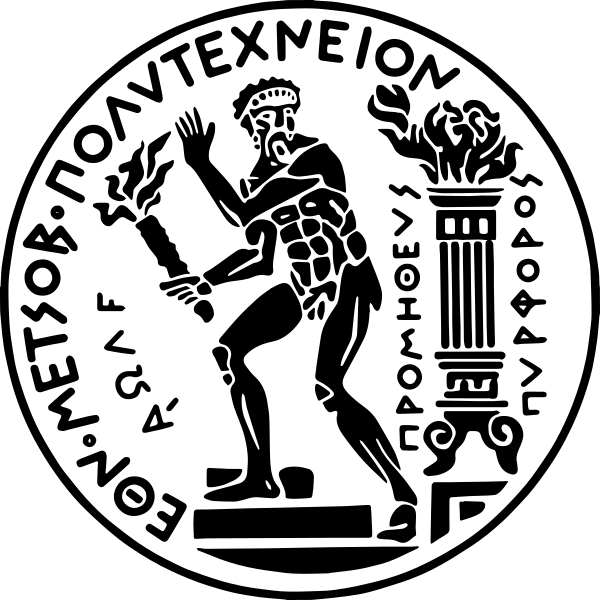
\includegraphics[width=\linewidth]{ntua_logo.png}
        \end{minipage}
        \hfill
        \begin{minipage}{0.65\textwidth}
            \centering
            {\LARGE \textbf{Εθνικό Μετσόβιο Πολυτεχνείο}}\\[0.3cm]
            {\large \textbf{Σχολή Ηλεκτρολόγων Μηχανικών \& Μηχανικών Υπολογιστών}}\\[0.2cm]
            \rule{\linewidth}{0.5pt}\\[0.3cm]
            {\large Εξάμηνο 8\textsuperscript{o}}\\[0.1cm]
            {\large \textbf{Όραση Υπολογιστών}}\\
        \end{minipage}

        \vspace{2cm}

        {\Huge \textbf{2η Εργαστηριακή Άσκηση}}\\[0.5cm]
        \rule{0.6\linewidth}{0.8pt}\\[0.5cm]
        {\LARGE \textbf{Εκτίμηση Οπτικής Ροής,\\[0.2cm]
        Εξαγωγή Χαρακτηριστικών σε Βίντεο\\[0.2cm]
        Αναγνώρισης Δράσεων,\\[0.2cm]
        Συνένωση Εικόνων}}\\[0.5cm]
        \rule{0.6\linewidth}{0.8pt}

        \vspace{2.5cm}

        {\large \textbf{Μέλη Ομάδας}}\\[0.6cm]
        \begin{tabular}{rl}
            \textbf{Καβαδάκης Σωτήρης}   & 03122035 \\[0.3cm]
            \textbf{Δαλαμπέκης Ιγνάτιος} & 03122017 \\
        \end{tabular}

        \vfill

        {\large Αθήνα, Απρίλιος 2026}

    \end{center}
\end{titlepage}
\clearpage

% ── Table of Contents ────────────────────────────────────────────────────────
\tableofcontents
\clearpage

% ─────────────────────────────────────────────────────────────────────────────
\section{Παρακολούθηση Προσώπου και Χεριών με Χρήση της Μεθόδου Οπτικής Ροής των Lucas-Kanade}

\subsection{Υλοποίηση του Αλγορίθμου των Lucas-Kanade}

% TODO

\subsection{Υπολογισμός της Μετατόπισης των Παραθύρων από τα Διανύσματα Οπτικής Ροής}

% TODO

\subsection{Πολυ-Κλιμακωτός Υπολογισμός Οπτικής Ροής}

% TODO

% ─────────────────────────────────────────────────────────────────────────────
\section{Εντοπισμός Χωρο-χρονικών Σημείων Ενδιαφέροντος και Εξαγωγή Χαρακτηριστικών σε Βίντεο Ανθρωπίνων Δράσεων}

Στο δεύτερο μέρος της άσκησης ασχολούμαστε με την εξαγωγή χωρο-χρονικών χαρακτηριστικών
από βίντεο ανθρωπίνων δράσεων σε grayscale, με στόχο την κατηγοριοποίησή τους σε μία εκ των τριών κλάσεων της βάσης KTH: (\textit{walking}, \textit{running},
\textit{handclapping}) της βάσης KTH. Η προσέγγιση βασίζεται
στη μεθοδολογία των Laptev et al.~\cite{laptev2008}, που εισάγει χωρο-χρονικά σημεία
ενδιαφέροντος και περιγραφητές HOG/HOF σε συνδυασμό με Bag-of-Words και SVM.

\subsection{Χωρο-χρονικά Σημεία Ενδιαφέροντος}

Ένα \textbf{χωρο-χρονικό σημείο ενδιαφέροντος} είναι ένα voxel $(x, y, t)$ του
βίντεο που χαρακτηρίζεται από σημαντική τοπική μεταβολή τόσο στον χωρικό
όσο και στον χρονικό άξονα. Διαισθητικά, μια ομαλή επιφάνεια του βίντεο δεν αποτελεί σημείο
ενδιαφέροντος ούτε στον χώρο ούτε στον χρόνο, ενώ μια ακμή που παραμένει στάσιμη
είναι ενδιαφέρουσα χωρικά αλλά όχι χρονικά. Μόνο οι περιοχές που εμφανίζουν
\emph{συγχρόνως} χωρική μεταβολή (γωνίες, αλλαγές κατεύθυνσης) και χρονική
μεταβολή (κίνηση, εμφάνιση και εξαφάνιση αντικειμένων) ικανοποιούν το κριτήριο
και επιλέγονται. Τα σημεία αυτά είναι πληροφοριακά πλούσια και ιδανικά ως βάση
για την εξαγωγή συμπαγών τοπικών περιγραφητών.

Υλοποιήθηκαν δύο ανιχνευτές: ο \textbf{Harris3D} και ο \textbf{Gabor}.

\subsubsection{Ανιχνευτής Harris3D}

Ο ανιχνευτής Harris3D~\cite{laptev2003} αποτελεί χωρο-χρονική επέκταση του
κλασικού ανιχνευτή γωνιών Harris-Stephens. Ο 2D Harris-Laplacian εντοπίζει χωρικές γωνίες
σε πολλαπλές κλίμακες ανεξαρτήτως κίνησης (αριστερά), ενώ ο Harris3D εντοπίζει σημεία που
πληρούν το κριτήριο γωνιότητας και στις τρεις διαστάσεις και συνεπώς είναι
πιο εστιασμένος στις δράσεις, λαμβάνοντας υπόψη και τη διάσταση του χρόνου (δεξιά). Η διαφορά τους φαίνεται εποπτικά στο Σχήμα~\ref{fig:harris_comparison}: 

\begin{figure}[H]
    \centering
    \begin{subfigure}[b]{0.48\textwidth}
        \centering
        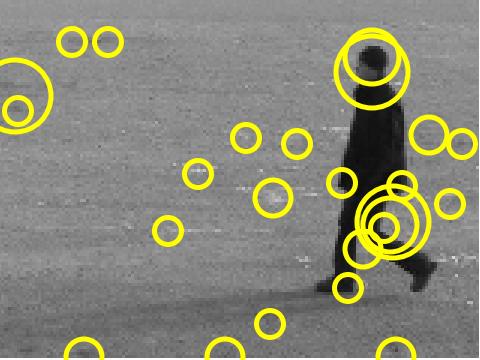
\includegraphics[width=\textwidth]{harris2d_multiscale.png}
        \caption{2D Harris-Laplacian (πολλαπλές κλίμακες)}
    \end{subfigure}
    \hfill
    \begin{subfigure}[b]{0.48\textwidth}
        \centering
        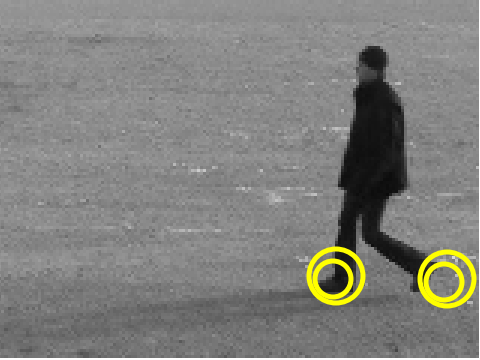
\includegraphics[width=\textwidth]{harris3d_multiscale.png}
        \caption{Harris3D (πολλαπλές κλίμακες)}
    \end{subfigure}
    \caption{Σύγκριση 2D Harris-Laplacian και Harris3D σε καρέ από βίντεο "walking" (KTH).
    Αριστερά: ο 2D ανιχνευτής εντοπίζει αφθονία γωνιών σε όλο το πλαίσιο: περιγράμματα,
    υφές και γωνίες φόντου, σε διαφορετικές χωρικές κλίμακες.
    Δεξιά: ο Harris3D επιλέγει πιο εστιασμένα σημεία, κυρίως στις
    περιοχή των άκρων που αφορά τον βηματσμό,
    φιλτράροντας ανενεργές περιοχές του φόντου.}
    \label{fig:harris_comparison}
\end{figure}

Όσον αφορά τον ανιχνευτή 3D Harris, η βασική ιδέα είναι: αν μετακινήσουμε
ένα μικρό χωρο-χρονικό παράθυρο γύρω από ένα voxel προς οποιαδήποτε κατεύθυνση
$(x, y, t)$, ένα σημείο ενδιαφέροντος είναι εκεί όπου η μεταβολή της έντασης
είναι μεγάλη για \emph{όλες} τις κατευθύνσεις. Αυτό κωδικοποιείται μέσω του
$3\times3$ δομικού τανυστή (second-moment matrix):
\begin{equation}
    \mathbf{M}(x,y,t;\,\sigma,\tau) = g(s\sigma,s\tau) \ast
    \begin{pmatrix}
        L_x^2    & L_x L_y & L_x L_t \\
        L_x L_y  & L_y^2   & L_y L_t \\
        L_x L_t  & L_y L_t & L_t^2
    \end{pmatrix}
\end{equation}
όπου $L = g(\sigma,\tau) \ast I$ είναι το βίντεο εξομαλυσμένο στην κλίμακα
διαφόρισης $(\sigma, \tau)$, οι παράγωγοι $L_x, L_y, L_t$ υπολογίζονται με τον
πυρήνα κεντρικών διαφορών $[-1,\,0,\,1]$ κατά τον αντίστοιχο άξονα, και
$g(s\sigma, s\tau)$ είναι ο γκαουσιανός πυρήνας κλίμακας ολοκλήρωσης
που εξομαλύνει τα γινόμενα παραγώγων. Η διάκριση των δύο κλιμάκων είναι
ουσιώδης: η κλίμακα διαφόρισης καθορίζει την ανάλυση στην οποία ανιχνεύονται οι
τοπικές μεταβολές, ενώ η κλίμακα ολοκλήρωσης ορίζει το χωρο-χρονικό γειτονικό
πλαίσιο μέσα στο οποίο αθροίζονται.
Ο πυρήνας $[-1,\,0,\,1]$ που χρησιμοποιούμε είναι ο απλούστερος πυρήνας κεντρικής διαφοράς πρώτης
τάξης: εκτιμά την παράγωγο στο κεντρικό σημείο χρησιμοποιώντας τους δύο γείτονές
του, χωρίς να εισάγει μετατόπιση φάσης.

Όταν και οι τρεις ιδιοτιμές του $\mathbf{M}$ είναι μεγάλες, το voxel αναγνωρίζεται
ως «γωνία» στον χωρο-χρόνο. Αντί για ρητό υπολογισμό ιδιοτιμών, χρησιμοποιείται
το αλγεβρικό κριτήριο:
\begin{equation}
    H(x,y,t) = \det(\mathbf{M}) - k \cdot \mathrm{trace}^3(\mathbf{M})
\end{equation}
Τα σημεία επιλέγονται με κατωφλίωση $H > \theta \cdot H_{\max}$, NMS σε γειτονιά
$3\times3\times3$ και διατήρηση των $N$ ισχυρότερων.

Ως προς την υλοποίηση, η 3D Gaussian εξομάλυνση εκτελείται ως τρεις διαδοχικές
\emph{1D} συνελίξεις κατά τους άξονες $x$, $y$, $t$ χωριστά, εκμεταλλευόμενη τη
διαχωρισιμότητα (separability) του γκαουσιανού πυρήνα. Επίσης, ο υπολογισμός του
$\det(\mathbf{M})$ γίνεται αναλυτικά μέσω της εκτεταμένης μορφής της $3\times3$
ορίζουσας, αποφεύγοντας αριθμητική αποσύνθεση σε ιδιοτιμές.

Αν και στη βιβλιογραφία \cite{laptev2008} προτείνεται πολυκλιμακική ανίχνευση (εξαγωγή σημείων σε πολλαπλές κλίμακες $(\sigma_i,\tau_j)$ για μείωση υπολογιστικού κόστους και ανεξαρτησία από σφάλματα επιλογής κλίμακας), στην παρούσα εργασία χρησιμοποιήθηκε ενιαία κλίμακα, εστιάζοντας στη μελέτη της επίδρασης των παραμέτρων $\sigma$, $\tau$ και $k$.

\subsubsection{Ανιχνευτής Gabor}

Ο ανιχνευτής Gabor αποτελεί χωρο-χρονική μέθοδο ανίχνευσης σημείων ενδιαφέροντος
βασισμένη σε φιλτράρισμα με τράπεζα φίλτρων Gabor. Σε αντίθεση με τον Harris3D, που
ανιχνεύει voxels με μεγάλη \emph{γεωμετρική} μεταβολή σε όλες τις κατευθύνσεις, ο
Gabor εστιάζει στην \emph{ενέργεια} τοπικής κίνησης: ανιχνεύει περιοχές που
παρουσιάζουν έντονη χρονική μεταβολή συγκεκριμένης χωροχρονικής συχνότητας. Αυτό τον κάνει
πιο «επιεική» ως προς τη χωρική γεωμετρία αλλά πιο εκλεκτικό ως προς τον
\emph{ρυθμό} της κίνησης, ιδιότητα ιδιαίτερα χρήσιμη για περιοδικές δράσεις
όπως βάδισμα και χειροκρότημα.

Η βασική ιδέα: ένα φίλτρο Gabor είναι επιλεκτικό τόσο ως προς τη χωρική / χρονική
\emph{κλίμακα} όσο και ως προς τη \emph{συχνότητα} κίνησης. Ορίζεται ως γκαουσιανή
περιβάλλουσα διαμορφωμένη από ημιτονοειδή φέρουσα:
\begin{equation}
    g_c(x,y,t;\,\sigma_x,\sigma_y,\sigma_t) =
    \frac{1}{(2\pi)^{3/2}\sigma_x\sigma_y\sigma_t}
    \exp\!\left[-\left(\frac{x^2}{2\sigma_x^2}+\frac{y^2}{2\sigma_y^2}+\frac{t^2}{2\sigma_t^2}\right)\right]
    \cos(\omega_{x_0}x + \omega_{y_0}y + \omega_{t_0}t)
\end{equation}
όπου $(\sigma_x,\sigma_y,\sigma_t)$ ορίζουν τη χωρο-χρονική κλίμακα (εύρος ζώνης) του
φίλτρου, και $(\omega_{x_0},\omega_{y_0},\omega_{t_0})$ είναι οι κεντρικές γωνιακές
συχνότητες στις οποίες αποκρίνεται. Στο πεδίο συχνοτήτων το φίλτρο έχει απόκριση
ζωνοπερατού φίλτρου: δύο Γκαουσιανοί όγκοι συγκεντρωμένοι γύρω από $\pm(\omega_{x_0},\omega_{y_0},\omega_{t_0})$.

Για κάθε κλίμακα $(\sigma, \tau)$ ορίζεται ένα \textbf{ζεύγος τετραγωνισμού}
(quadrature pair) — ένα άρτιο φίλτρο (συνημίτονο) και ένα περιττό (ημίτονο):
\begin{align}
    h_{\text{ev}}(t;\,\tau) &= \cos(2\pi \omega t)\cdot g(t;\,\tau), &
    h_{\text{od}}(t;\,\tau) &= \sin(2\pi \omega t)\cdot g(t;\,\tau)
\end{align}
όπου $g(t;\tau) = \exp\!\bigl(-t^2/(2\tau^2)\bigr)$ και $\omega = 4/\tau$.
Τα φίλτρα κανονικοποιούνται ως προς τη νόρμα $L_1$ και εκτείνονται σε
$t \in [-2\tau, 2\tau]$. Το ζεύγος αξιοποιεί την ιδιότητα ότι $\cos^2\!+\sin^2\!=1$:
η συνδυασμένη ενέργεια εξόδου δεν εξαρτάται από τη χρονική φάση της κίνησης, άρα
ανιχνεύει ρυθμικά κινούμενες δομές ανεξαρτήτως της στιγμής μέτρησης.

Η σχέση $\omega = 4/\tau$ δεν είναι τυχαία: εξασφαλίζει ότι στο χρονικό παράθυρο
$[-2\tau, 2\tau]$ χωράνε ακριβώς \emph{δύο πλήρεις ταλαντώσεις} της ημιτονοειδούς
φέρουσας. Αυτό διατηρεί τo φίλτρο ανταποκρινόμενο σε ένα σαφώς ορισμένο εύρος
χρονικών συχνοτήτων: αρκετά στενό ώστε να είναι εκλεκτικό, αρκετά πλατύ ώστε
να μην απαιτεί ακριβή συγχρονισμό με τον ρυθμό κίνησης.

Το κριτήριο ανίχνευσης είναι το άθροισμα τετραγώνων των δύο αποκρίσεων:
\begin{equation}
    H(x,y,t) =
    \bigl(I \ast h_{\text{ev}}\bigr)^2(x,y,t) +
    \bigl(I \ast h_{\text{od}}\bigr)^2(x,y,t)
\end{equation}

Όσον αφορά την υλοποίηση του, εκμεταλλευόμαστε τη \emph{διαχωρισιμότητα} του 3D φίλτρου
Gabor: χωρική εξομάλυνση (2D Gaussian, κλίμακα $\sigma$) και χρονική συνέλιξη
(1D Gabor, κλίμακα $\tau$) εκτελούνται ανεξάρτητα κατά τους αντίστοιχους άξονες,
μειώνοντας σημαντικά το υπολογιστικό κόστος. Σημειώνεται ότι στο πλήρες 3D μοντέλο
(εξ.~παραπάνω) το χωρικό τμήμα του φίλτρου έχει και χωρικές συχνότητες
$(\omega_{x_0}, \omega_{y_0}) \neq 0$, δηλαδή είναι \emph{προσανατολισμένο} στον
χώρο. Στην υλοποίησή μας ο χωρικός προσανατολισμός αφαιρείται θέτοντας
$\omega_{x_0}\!=\!\omega_{y_0}\!=\!0$, οπότε η χωρική συνιστώσα εκφυλίζεται σε
ισότροπη Γκαουσιανή εξομάλυνση — απλοποίηση που μειώνει το μέγεθος της τράπεζας
φίλτρων αλλά χάνει την ευαισθησία σε χωρική κατεύθυνση κίνησης.

\subsubsection{Απόρριψη Ομαλών Περιοχών και Επιλογή Σημείων}

Και οι δύο ανιχνευτές ακολουθούν κοινή στρατηγική επιλογής σημείων:
\begin{enumerate}
    \item \textbf{Κατωφλίωση}: διατηρούνται μόνο voxels με
          $H(x,y,t) > \theta \cdot H_{\max}$, ώστε να απορριφθούν ομαλές
          ή χαμηλής ενέργειας περιοχές. Η παράμετρος $\theta$ ελέγχει
          πόσο αυστηρή είναι αυτή η απόρριψη.
    \item \textbf{Non-maximum suppression (NMS)}: κρατούνται μόνο τα τοπικά
          μέγιστα σε γειτονιά $3\times3\times3$ voxels, εξασφαλίζοντας
          χωρο-χρονικά διαχωρισμένα σημεία.
    \item \textbf{Επιλογή top-$N$}: από τα εναπομείναντα σημεία επιλέγονται
          τα $N$ με τη μεγαλύτερη τιμή απόκρισης $H$.
\end{enumerate}

\subsubsection{Απεικόνιση Σημείων Ενδιαφέροντος και Σχολιασμός}

Για κάθε ανιχνευτή (Harris3D, Gabor) οπτικοποιήθηκαν η απόκριση $H$ και τα
εντοπισμένα σημεία για ένα αντιπροσωπευτικό βίντεο ανά κλάση δράσης
(\textit{walking}, \textit{running}, \textit{handclapping}), με παραμέτρους
$\sigma{=}2$, $\tau{=}1.5$, $\theta{=}0.1$, $N{=}500$.

Για κάθε κλάση παρουσιάζονται διαδοχικά: Harris3D εντοπισμός, Harris3D heatmap,
Gabor εντοπισμός, Gabor heatmap, σε τρία αντιπροσωπευτικά frames.

% ══ walking ════════════════════════════════════════════════════════════════════
\begin{figure}[H]
    \centering
    \begin{subfigure}[b]{0.32\textwidth}
        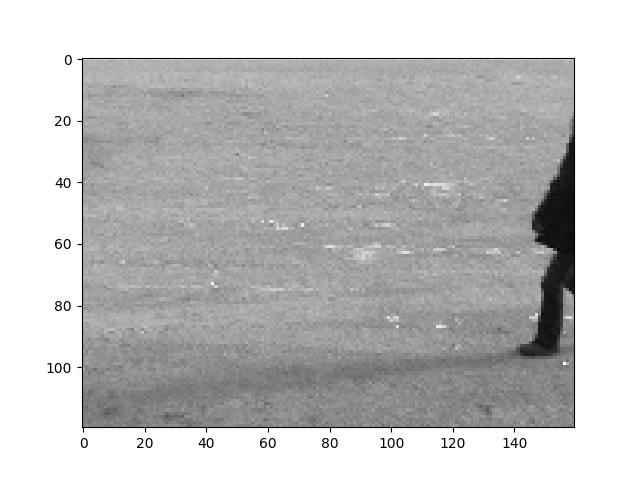
\includegraphics[width=\textwidth]{walking_harris_s2_t1.5_thr0.01_frame12_det.png}
        \caption{frame 12}
    \end{subfigure}
    \hfill
    \begin{subfigure}[b]{0.32\textwidth}
        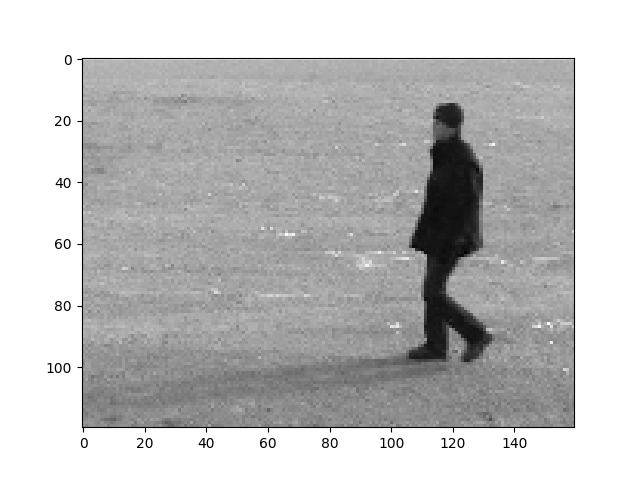
\includegraphics[width=\textwidth]{walking_harris_s2_t1.5_thr0.01_frame27_det.png}
        \caption{frame 27}
    \end{subfigure}
    \hfill
    \begin{subfigure}[b]{0.32\textwidth}
        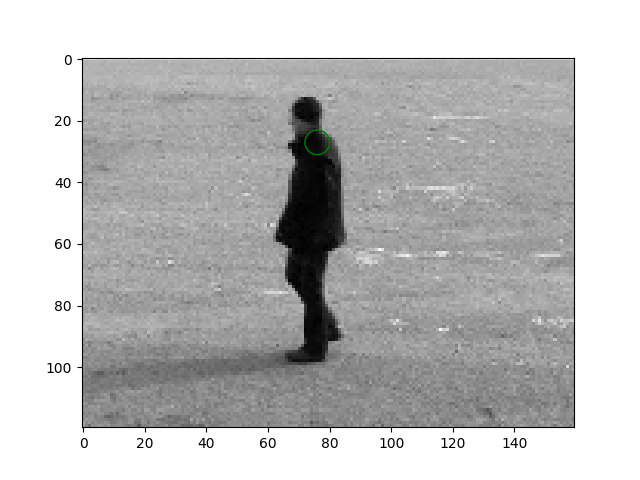
\includegraphics[width=\textwidth]{walking_harris_s2_t1.5_thr0.01_frame42_det.png}
        \caption{frame 42}
    \end{subfigure}
    \caption{Harris3D - walking: εντοπισμένα σημεία ενδιαφέροντος.}
    \label{fig:harris_det_walking}
\end{figure}

\begin{figure}[H]
    \centering
    \begin{subfigure}[b]{0.32\textwidth}
        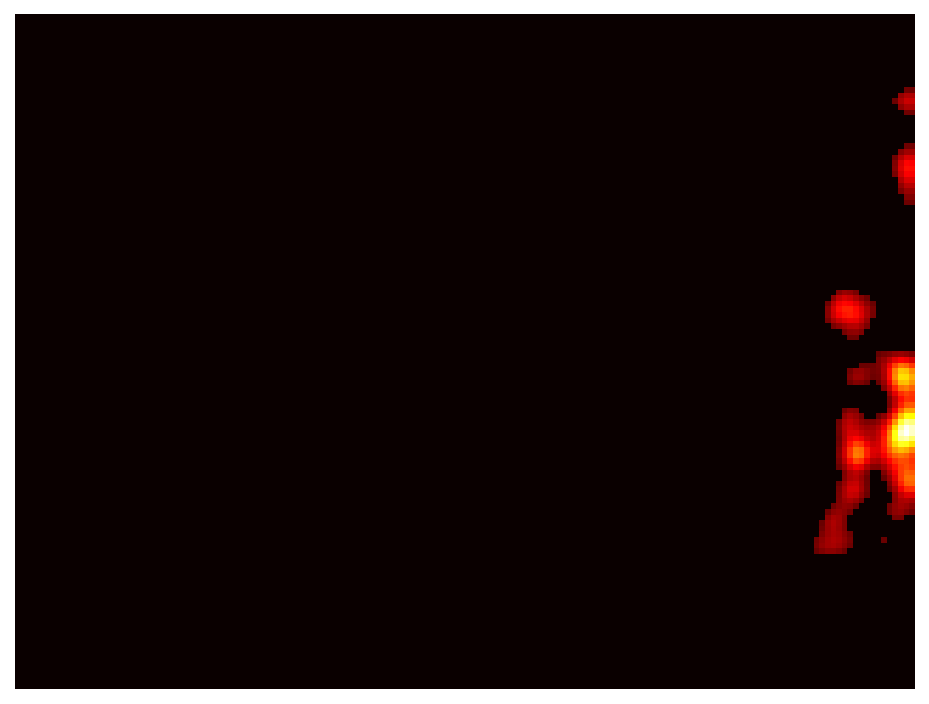
\includegraphics[width=\textwidth]{walking_harris_s2_t1.5_thr0.01_frame12_H.png}
        \caption{frame 12}
    \end{subfigure}
    \hfill
    \begin{subfigure}[b]{0.32\textwidth}
        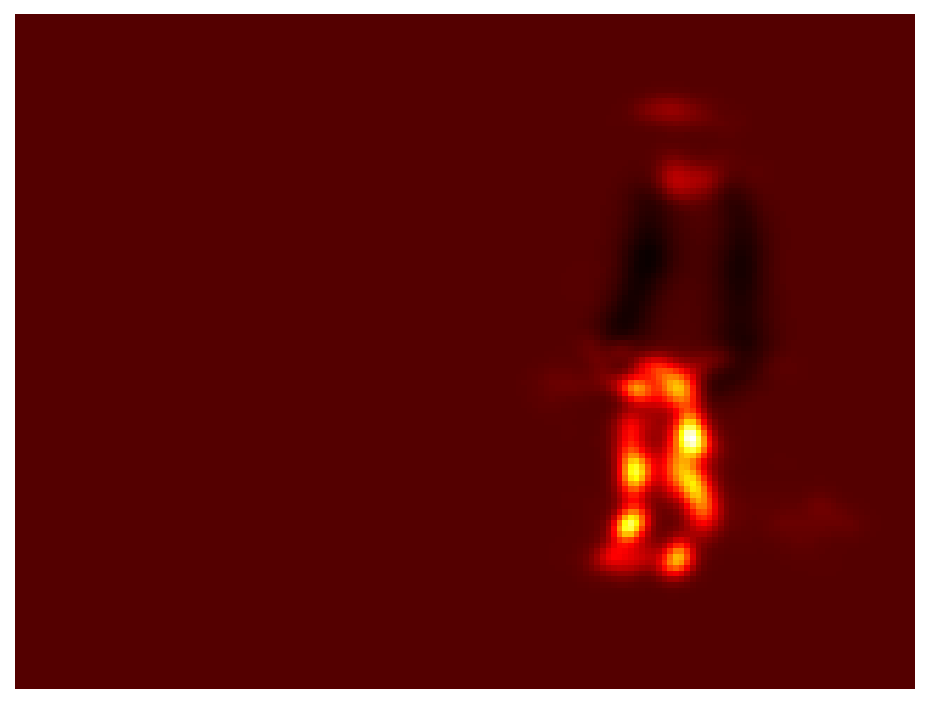
\includegraphics[width=\textwidth]{walking_harris_s2_t1.5_thr0.01_frame27_H.png}
        \caption{frame 27}
    \end{subfigure}
    \hfill
    \begin{subfigure}[b]{0.32\textwidth}
        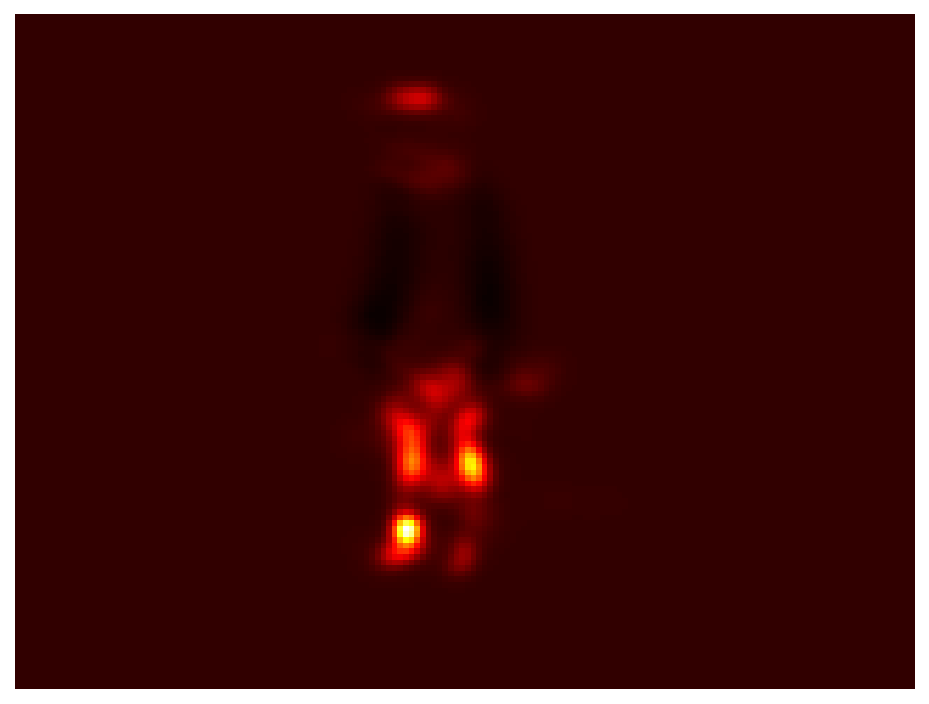
\includegraphics[width=\textwidth]{walking_harris_s2_t1.5_thr0.01_frame42_H.png}
        \caption{frame 42}
    \end{subfigure}
    \caption{Harris3D - walking: χάρτης απόκρισης $H$ (κλίμακα \textit{hot}).}
    \label{fig:harris_H_walking}
\end{figure}

\begin{figure}[H]
    \centering
    \begin{subfigure}[b]{0.32\textwidth}
        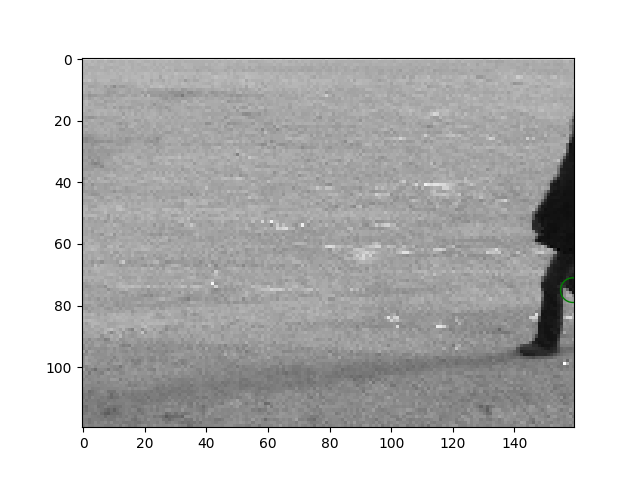
\includegraphics[width=\textwidth]{walking_gabor_s2_t1.5_thr0.1_frame12_det.png}
        \caption{frame 12}
    \end{subfigure}
    \hfill
    \begin{subfigure}[b]{0.32\textwidth}
        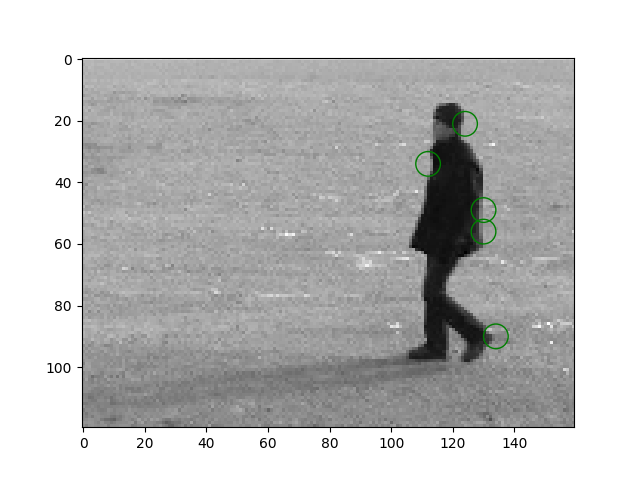
\includegraphics[width=\textwidth]{walking_gabor_s2_t1.5_thr0.1_frame27_det.png}
        \caption{frame 27}
    \end{subfigure}
    \hfill
    \begin{subfigure}[b]{0.32\textwidth}
        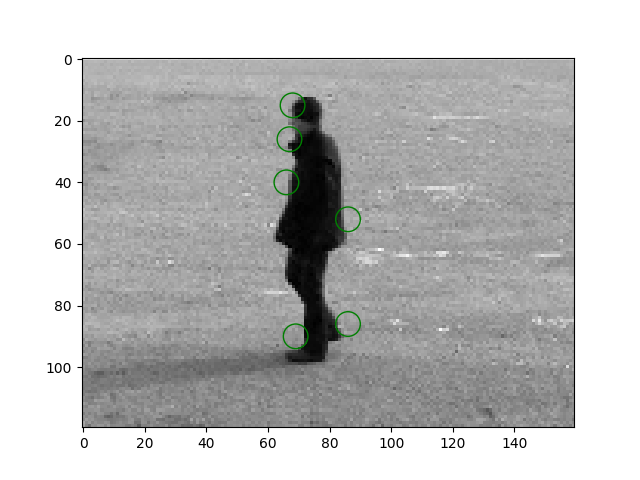
\includegraphics[width=\textwidth]{walking_gabor_s2_t1.5_thr0.1_frame42_det.png}
        \caption{frame 42}
    \end{subfigure}
    \caption{Gabor - walking: εντοπισμένα σημεία ενδιαφέροντος.}
    \label{fig:gabor_det_walking}
\end{figure}

\begin{figure}[H]
    \centering
    \begin{subfigure}[b]{0.32\textwidth}
        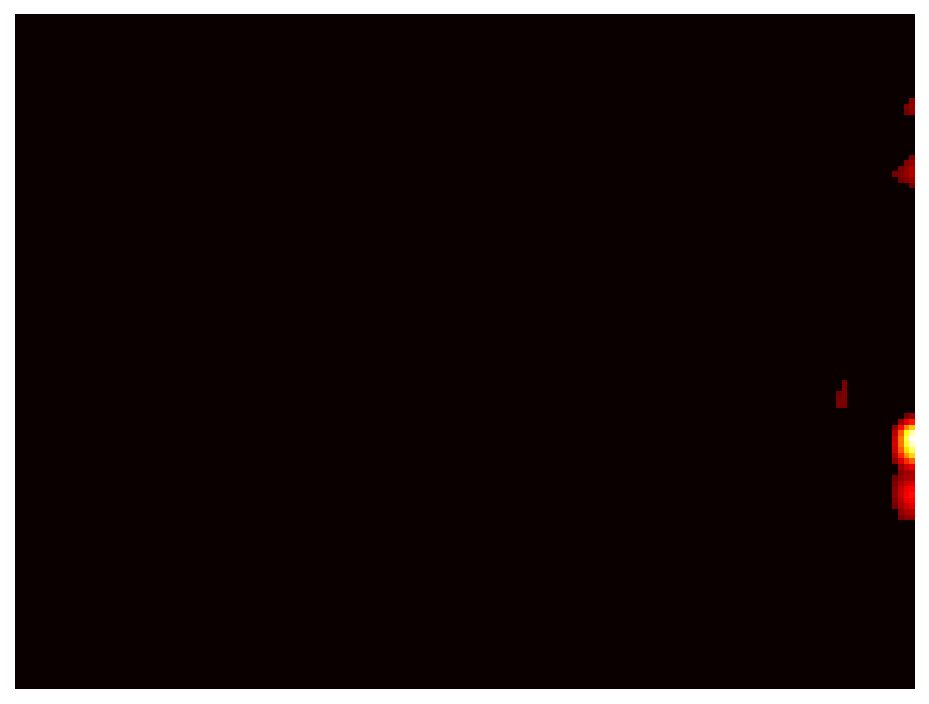
\includegraphics[width=\textwidth]{walking_gabor_s2_t1.5_thr0.1_frame12_H.png}
        \caption{frame 12}
    \end{subfigure}
    \hfill
    \begin{subfigure}[b]{0.32\textwidth}
        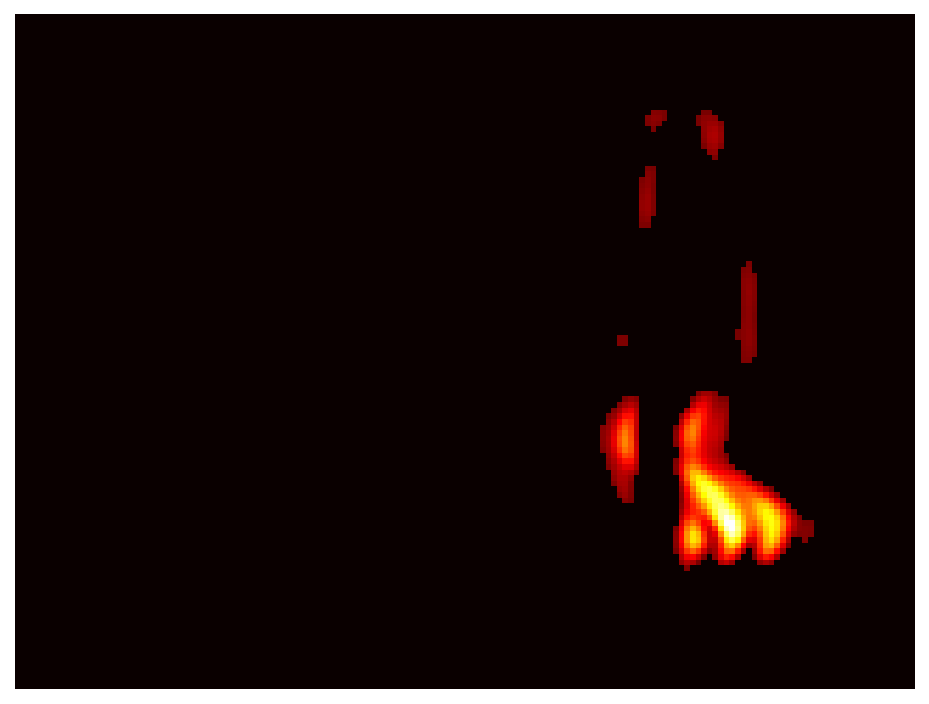
\includegraphics[width=\textwidth]{walking_gabor_s2_t1.5_thr0.1_frame27_H.png}
        \caption{frame 27}
    \end{subfigure}
    \hfill
    \begin{subfigure}[b]{0.32\textwidth}
        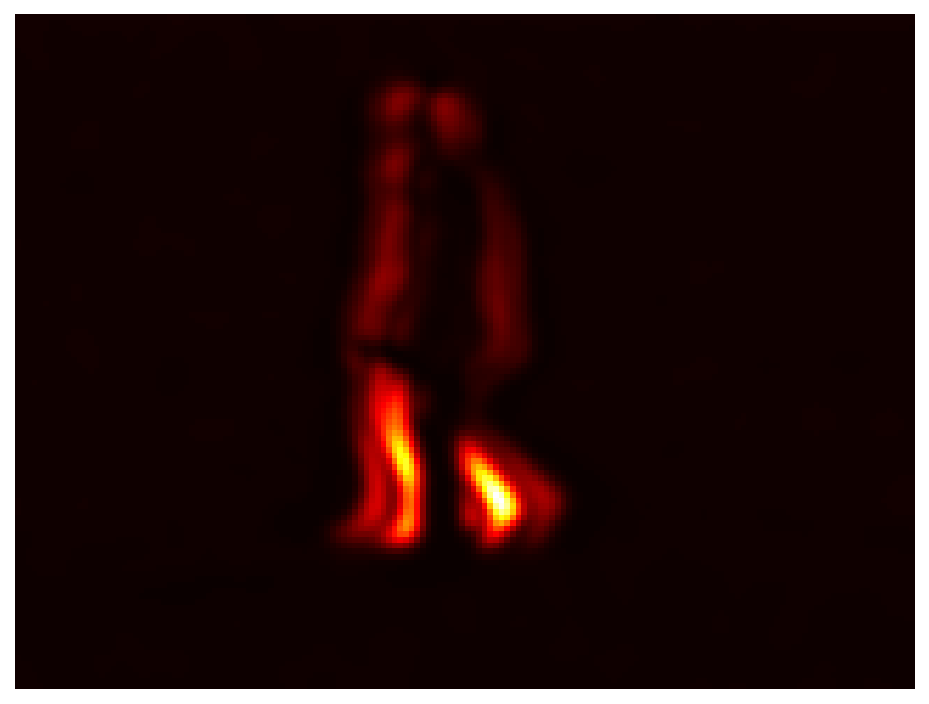
\includegraphics[width=\textwidth]{walking_gabor_s2_t1.5_thr0.1_frame42_H.png}
        \caption{frame 42}
    \end{subfigure}
    \caption{Gabor - walking: χάρτης ενέργειας $H$ (κλίμακα \textit{hot}).}
    \label{fig:gabor_H_walking}
\end{figure}

% ══ running ════════════════════════════════════════════════════════════════════
\begin{figure}[H]
    \centering
    \begin{subfigure}[b]{0.32\textwidth}
        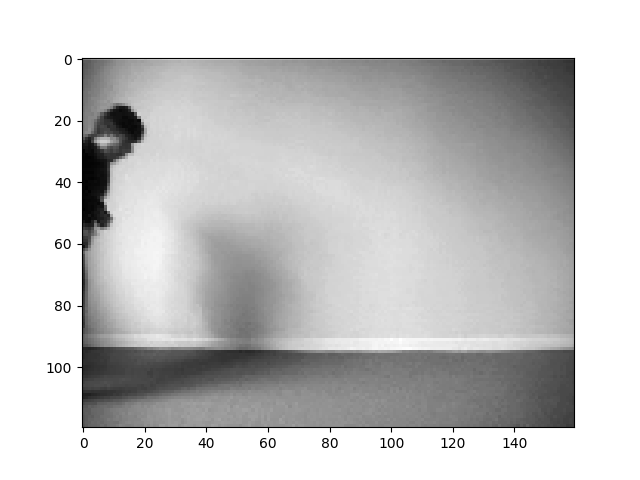
\includegraphics[width=\textwidth]{running_harris_s2_t1.5_thr0.01_frame12_det.png}
        \caption{frame 12}
    \end{subfigure}
    \hfill
    \begin{subfigure}[b]{0.32\textwidth}
        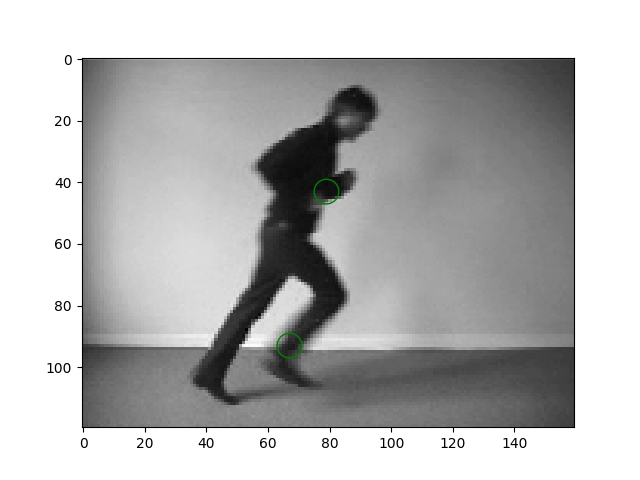
\includegraphics[width=\textwidth]{running_harris_s2_t1.5_thr0.01_frame27_det.png}
        \caption{frame 27}
    \end{subfigure}
    \hfill
    \begin{subfigure}[b]{0.32\textwidth}
        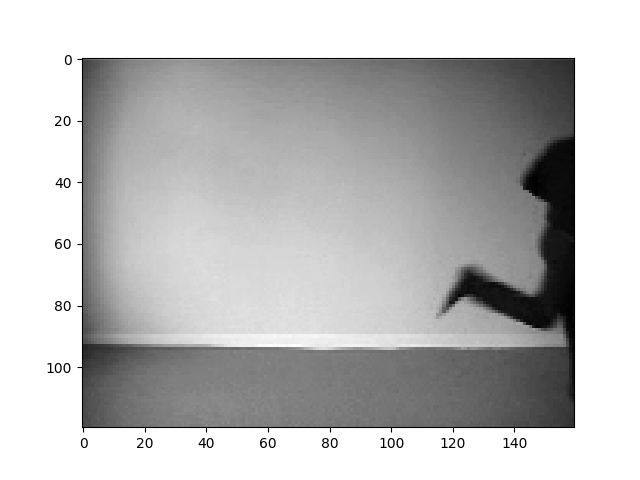
\includegraphics[width=\textwidth]{running_harris_s2_t1.5_thr0.01_frame42_det.png}
        \caption{frame 42}
    \end{subfigure}
    \caption{Harris3D - running: εντοπισμένα σημεία ενδιαφέροντος.}
    \label{fig:harris_det_running}
\end{figure}

\begin{figure}[H]
    \centering
    \begin{subfigure}[b]{0.32\textwidth}
        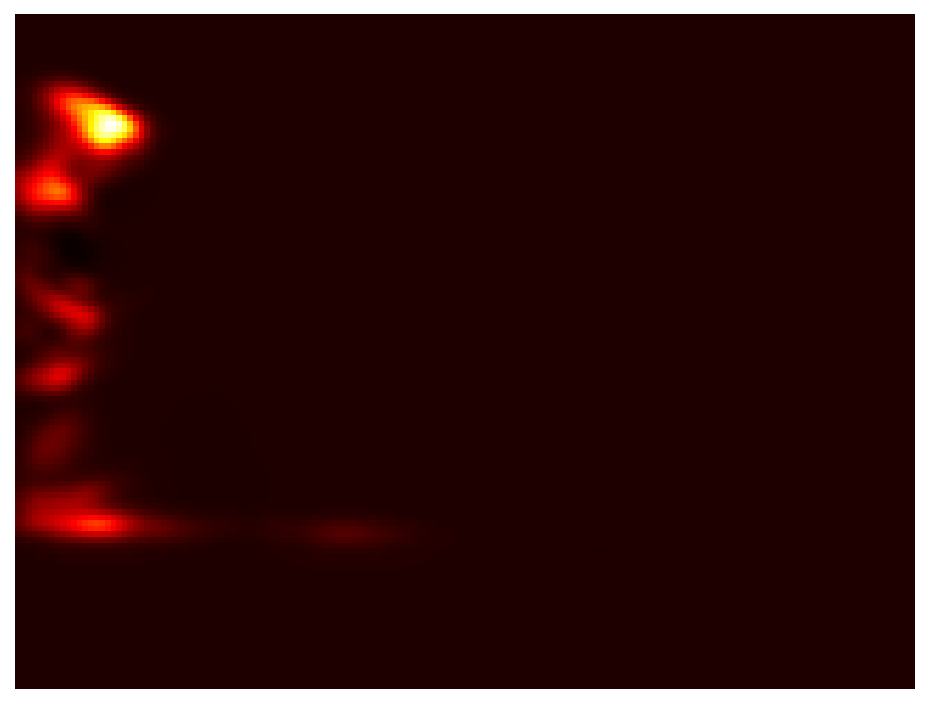
\includegraphics[width=\textwidth]{running_harris_s2_t1.5_thr0.01_frame12_H.png}
        \caption{frame 12}
    \end{subfigure}
    \hfill
    \begin{subfigure}[b]{0.32\textwidth}
        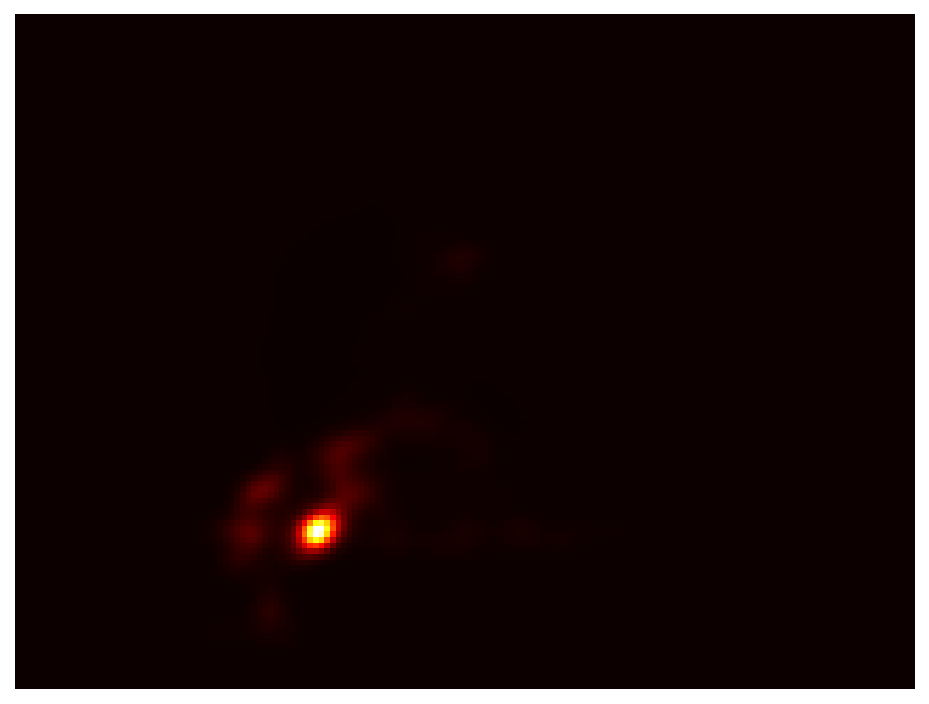
\includegraphics[width=\textwidth]{running_harris_s2_t1.5_thr0.01_frame27_H.png}
        \caption{frame 27}
    \end{subfigure}
    \hfill
    \begin{subfigure}[b]{0.32\textwidth}
        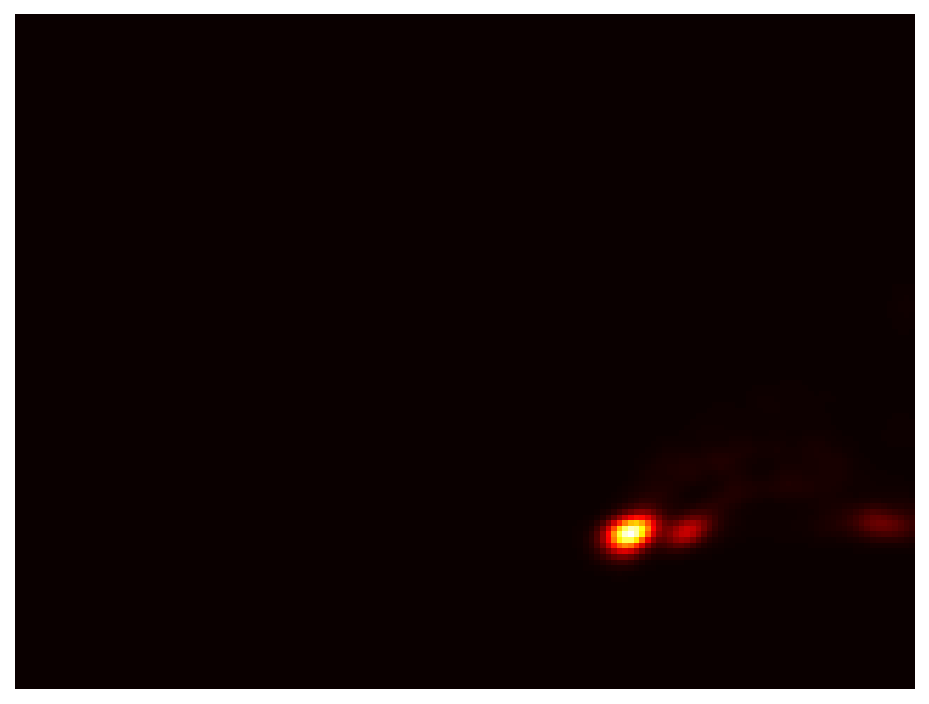
\includegraphics[width=\textwidth]{running_harris_s2_t1.5_thr0.01_frame42_H.png}
        \caption{frame 42}
    \end{subfigure}
    \caption{Harris3D - running: χάρτης απόκρισης $H$ (κλίμακα \textit{hot}).}
    \label{fig:harris_H_running}
\end{figure}

\begin{figure}[H]
    \centering
    \begin{subfigure}[b]{0.32\textwidth}
        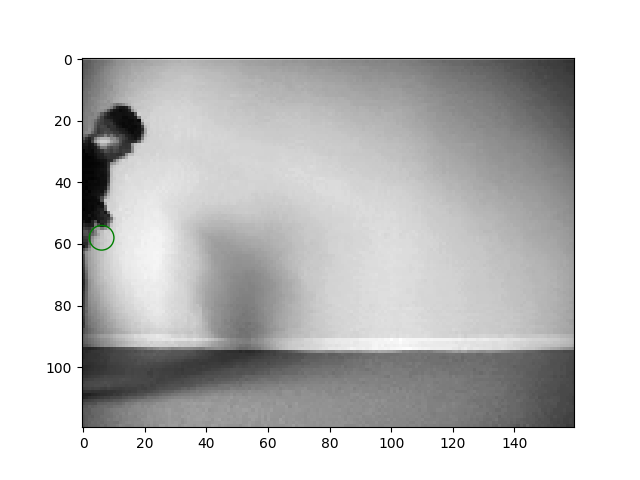
\includegraphics[width=\textwidth]{running_gabor_s2_t1.5_thr0.1_frame12_det.png}
        \caption{frame 12}
    \end{subfigure}
    \hfill
    \begin{subfigure}[b]{0.32\textwidth}
        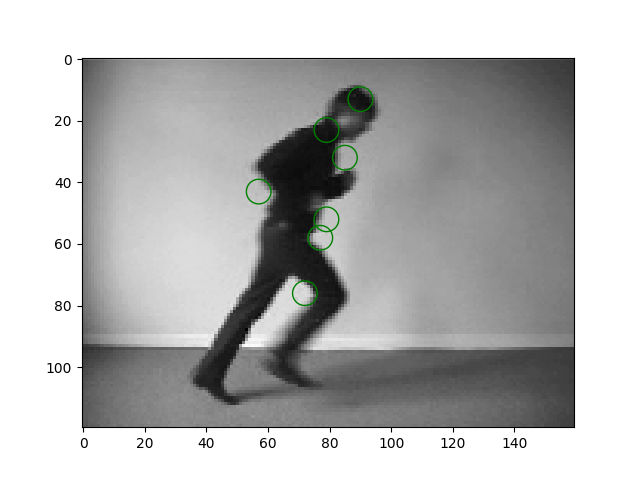
\includegraphics[width=\textwidth]{running_gabor_s2_t1.5_thr0.1_frame27_det.png}
        \caption{frame 27}
    \end{subfigure}
    \hfill
    \begin{subfigure}[b]{0.32\textwidth}
        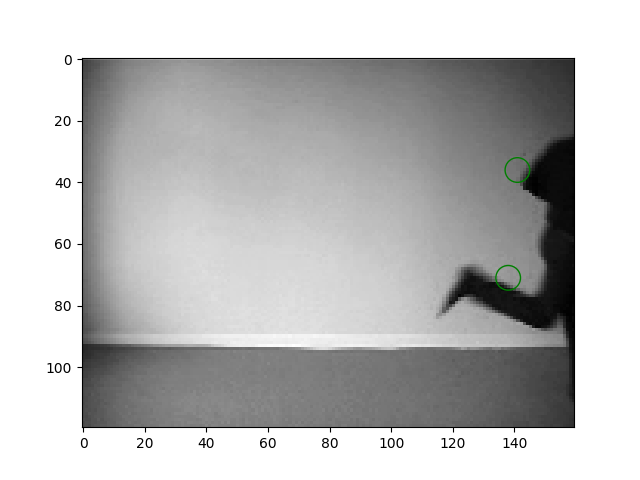
\includegraphics[width=\textwidth]{running_gabor_s2_t1.5_thr0.1_frame42_det.png}
        \caption{frame 42}
    \end{subfigure}
    \caption{Gabor - running: εντοπισμένα σημεία ενδιαφέροντος.}
    \label{fig:gabor_det_running}
\end{figure}

\begin{figure}[H]
    \centering
    \begin{subfigure}[b]{0.32\textwidth}
        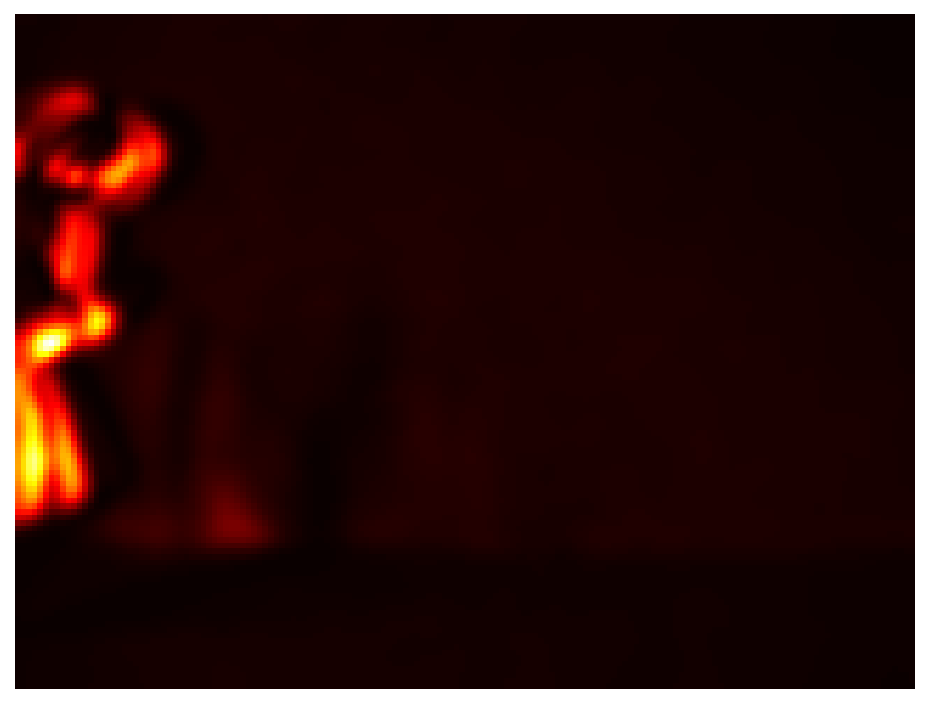
\includegraphics[width=\textwidth]{running_gabor_s2_t1.5_thr0.1_frame12_H.png}
        \caption{frame 12}
    \end{subfigure}
    \hfill
    \begin{subfigure}[b]{0.32\textwidth}
        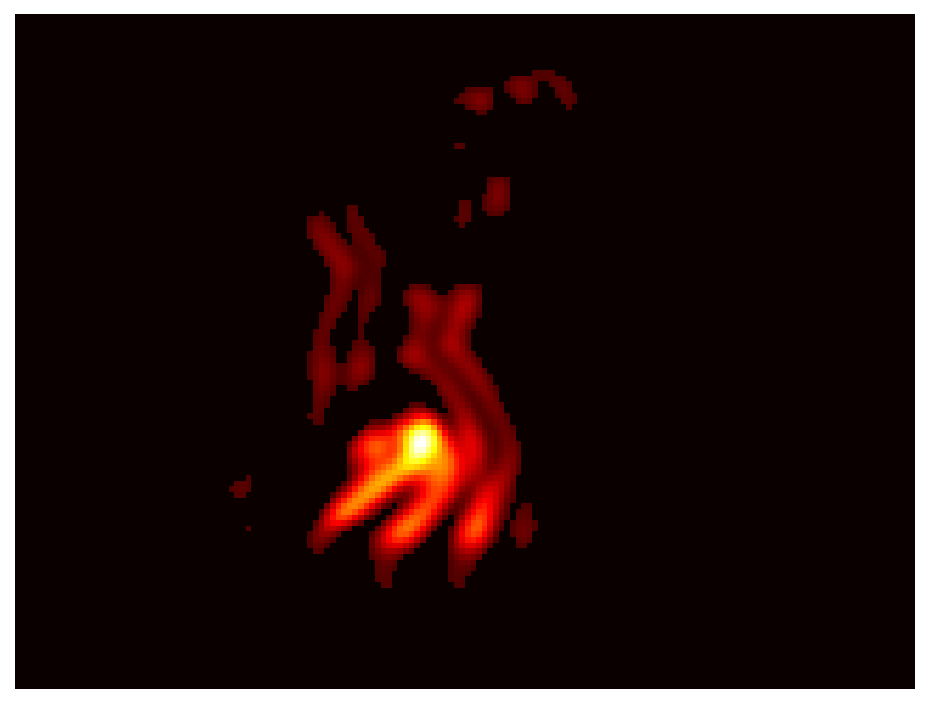
\includegraphics[width=\textwidth]{running_gabor_s2_t1.5_thr0.1_frame27_H.png}
        \caption{frame 27}
    \end{subfigure}
    \hfill
    \begin{subfigure}[b]{0.32\textwidth}
        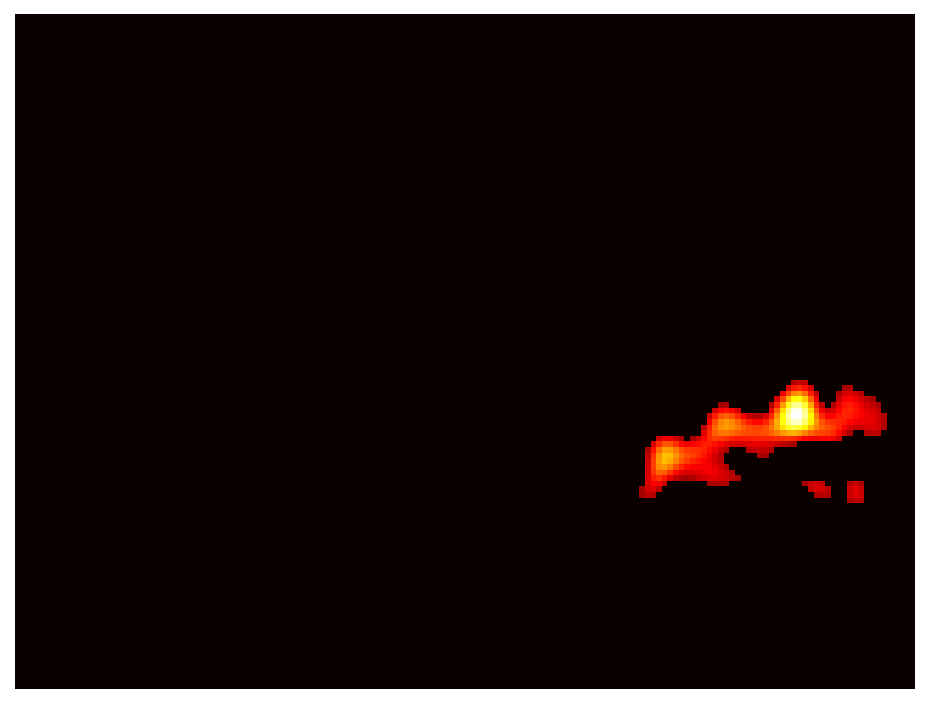
\includegraphics[width=\textwidth]{running_gabor_s2_t1.5_thr0.1_frame42_H.png}
        \caption{frame 42}
    \end{subfigure}
    \caption{Gabor - running: χάρτης ενέργειας $H$ (κλίμακα \textit{hot}).}
    \label{fig:gabor_H_running}
\end{figure}

% ══ handclapping ═══════════════════════════════════════════════════════════════
\begin{figure}[H]
    \centering
    \begin{subfigure}[b]{0.32\textwidth}
        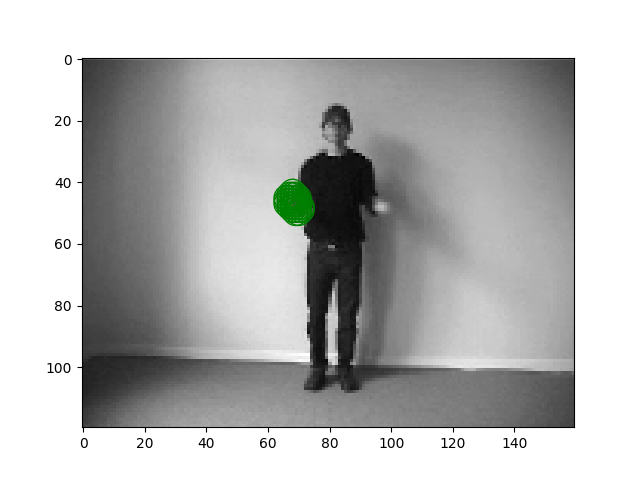
\includegraphics[width=\textwidth]{handclapping_harris_s2_t1.5_thr0.01_frame12_det.png}
        \caption{frame 12}
    \end{subfigure}
    \hfill
    \begin{subfigure}[b]{0.32\textwidth}
        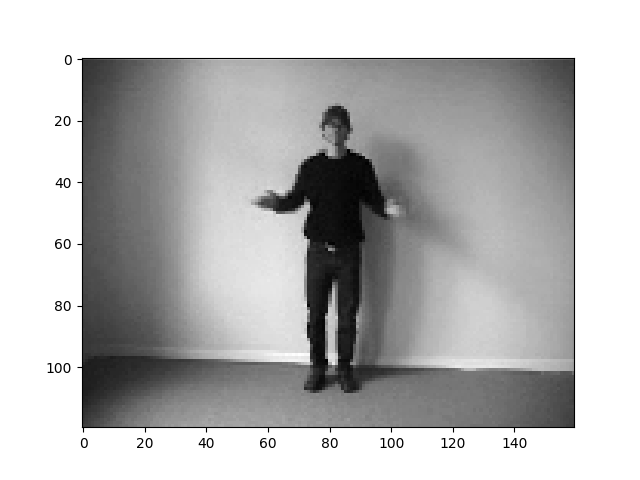
\includegraphics[width=\textwidth]{handclapping_harris_s2_t1.5_thr0.01_frame27_det.png}
        \caption{frame 27}
    \end{subfigure}
    \hfill
    \begin{subfigure}[b]{0.32\textwidth}
        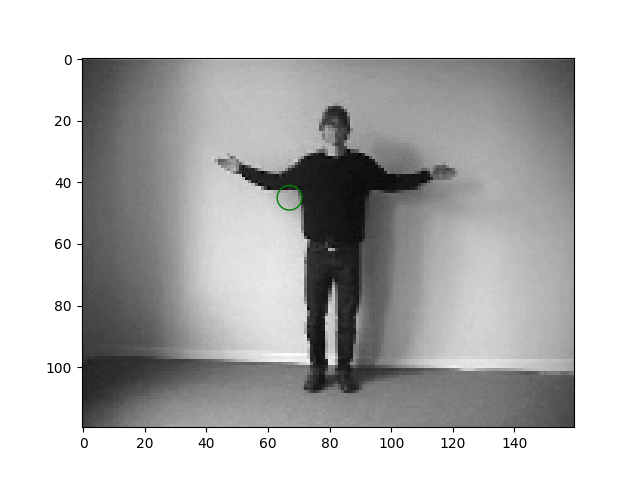
\includegraphics[width=\textwidth]{handclapping_harris_s2_t1.5_thr0.01_frame42_det.png}
        \caption{frame 42}
    \end{subfigure}
    \caption{Harris3D - handclapping: εντοπισμένα σημεία ενδιαφέροντος.}
    \label{fig:harris_det_handclapping}
\end{figure}

\begin{figure}[H]
    \centering
    \begin{subfigure}[b]{0.32\textwidth}
        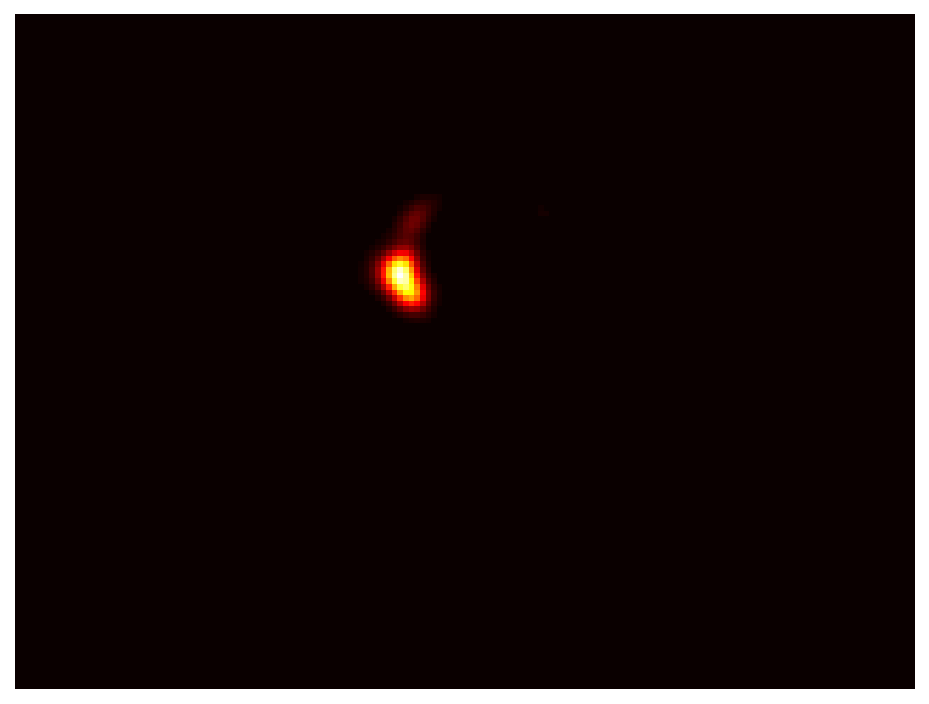
\includegraphics[width=\textwidth]{handclapping_harris_s2_t1.5_thr0.01_frame12_H.png}
        \caption{frame 12}
    \end{subfigure}
    \hfill
    \begin{subfigure}[b]{0.32\textwidth}
        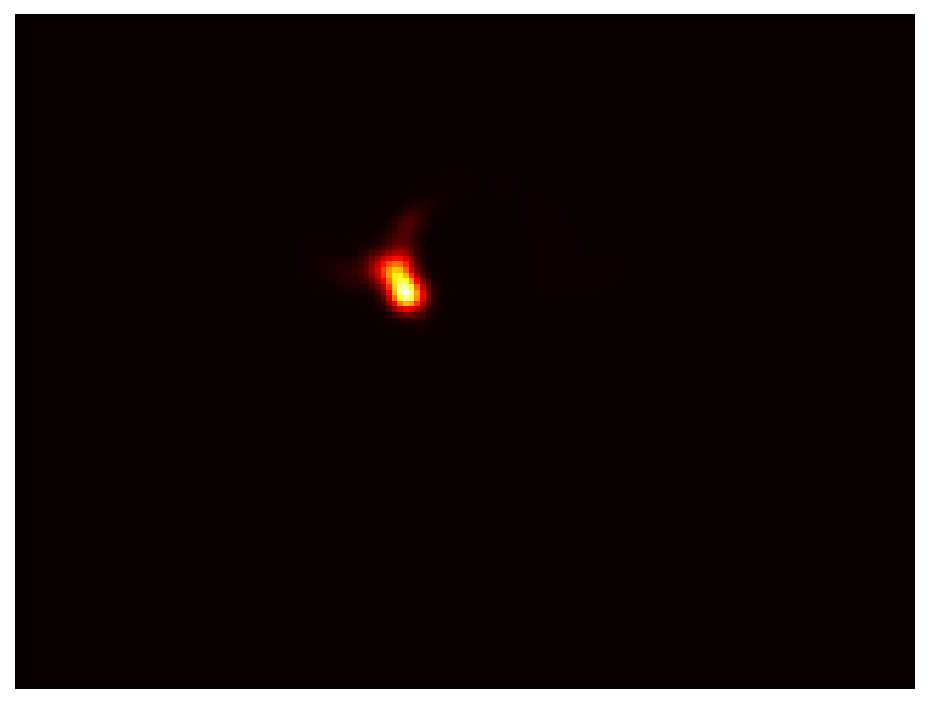
\includegraphics[width=\textwidth]{handclapping_harris_s2_t1.5_thr0.01_frame27_H.png}
        \caption{frame 27}
    \end{subfigure}
    \hfill
    \begin{subfigure}[b]{0.32\textwidth}
        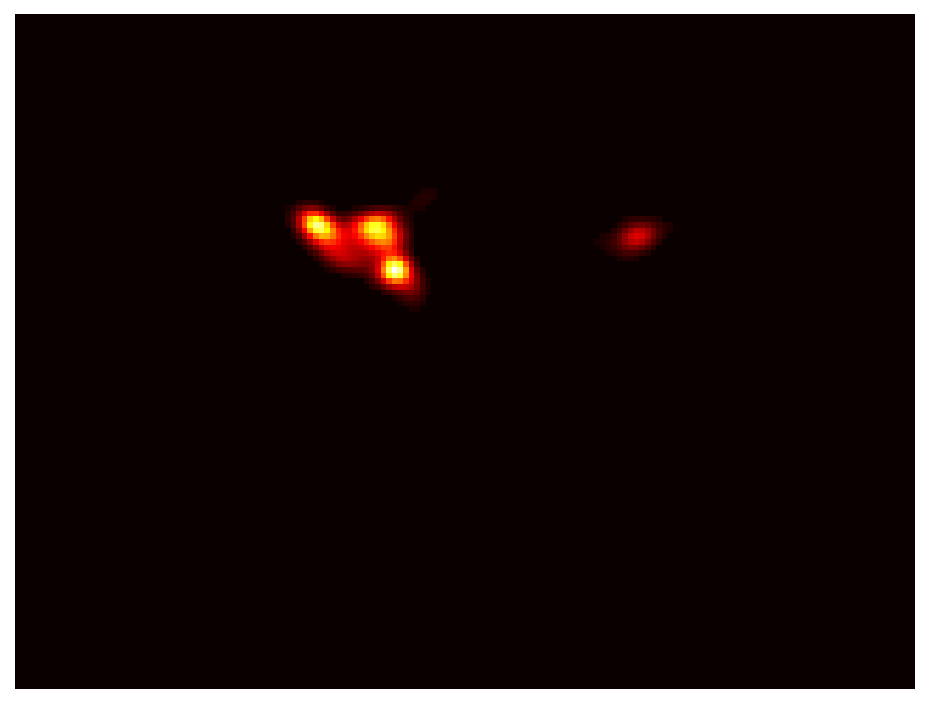
\includegraphics[width=\textwidth]{handclapping_harris_s2_t1.5_thr0.01_frame42_H.png}
        \caption{frame 42}
    \end{subfigure}
    \caption{Harris3D - handclapping: χάρτης απόκρισης $H$ (κλίμακα \textit{hot}).}
    \label{fig:harris_H_handclapping}
\end{figure}

\begin{figure}[H]
    \centering
    \begin{subfigure}[b]{0.32\textwidth}
        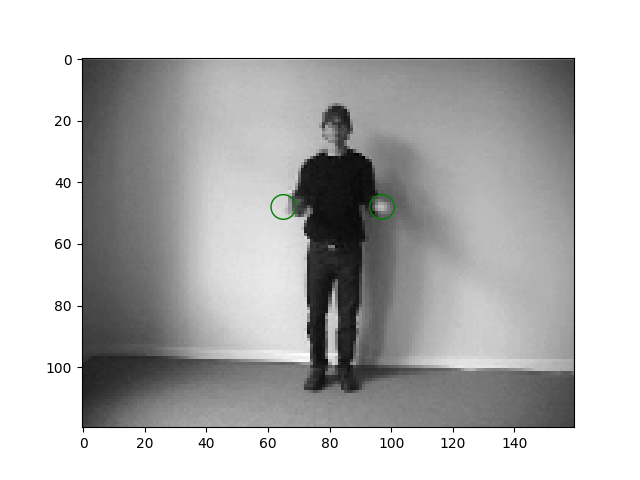
\includegraphics[width=\textwidth]{handclapping_gabor_s2_t1.5_thr0.1_frame12_det.png}
        \caption{frame 12}
    \end{subfigure}
    \hfill
    \begin{subfigure}[b]{0.32\textwidth}
        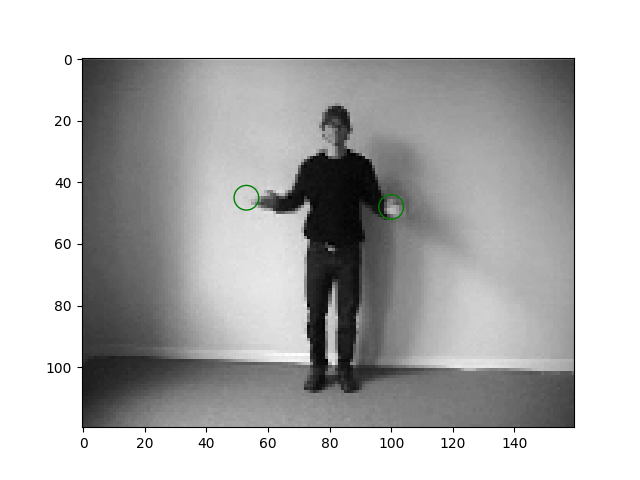
\includegraphics[width=\textwidth]{handclapping_gabor_s2_t1.5_thr0.1_frame27_det.png}
        \caption{frame 27}
    \end{subfigure}
    \hfill
    \begin{subfigure}[b]{0.32\textwidth}
        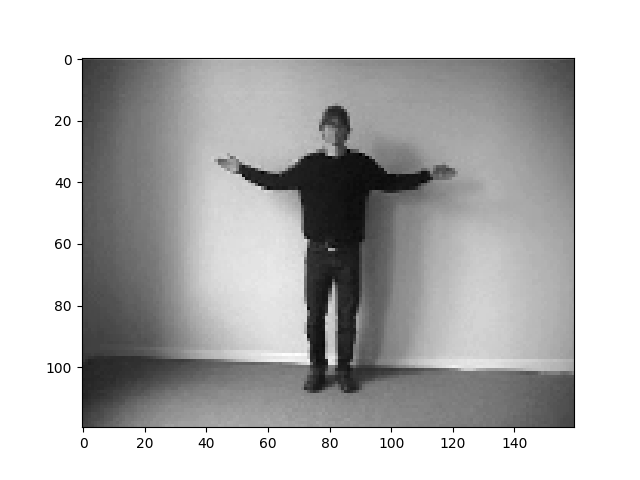
\includegraphics[width=\textwidth]{handclapping_gabor_s2_t1.5_thr0.1_frame42_det.png}
        \caption{frame 42}
    \end{subfigure}
    \caption{Gabor - handclapping: εντοπισμένα σημεία ενδιαφέροντος.}
    \label{fig:gabor_det_handclapping}
\end{figure}

\begin{figure}[H]
    \centering
    \begin{subfigure}[b]{0.32\textwidth}
        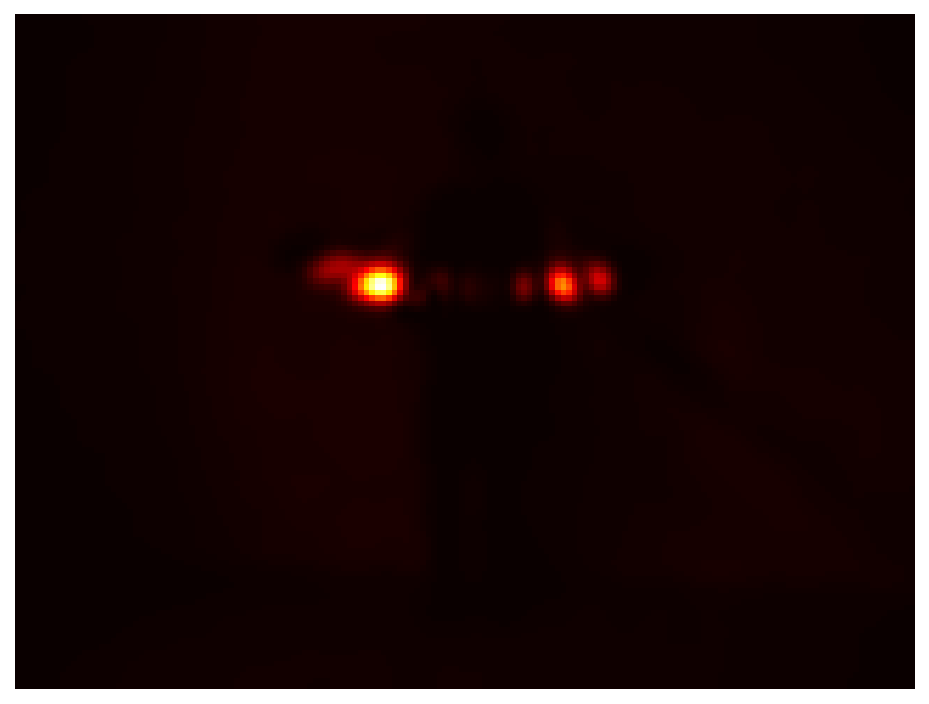
\includegraphics[width=\textwidth]{handclapping_gabor_s2_t1.5_thr0.1_frame12_H.png}
        \caption{frame 12}
    \end{subfigure}
    \hfill
    \begin{subfigure}[b]{0.32\textwidth}
        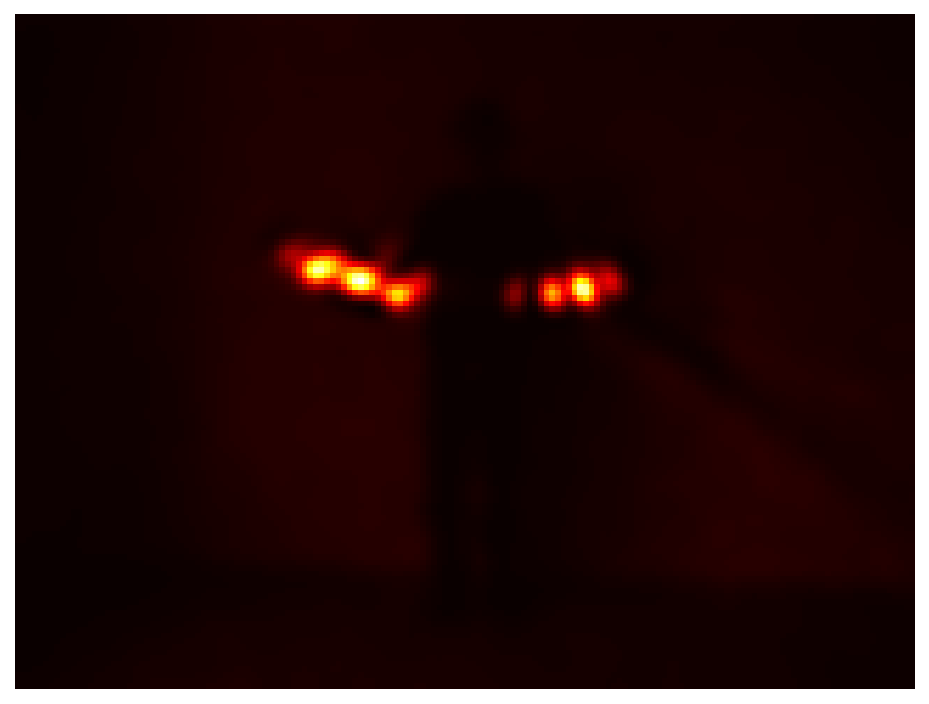
\includegraphics[width=\textwidth]{handclapping_gabor_s2_t1.5_thr0.1_frame27_H.png}
        \caption{frame 27}
    \end{subfigure}
    \hfill
    \begin{subfigure}[b]{0.32\textwidth}
        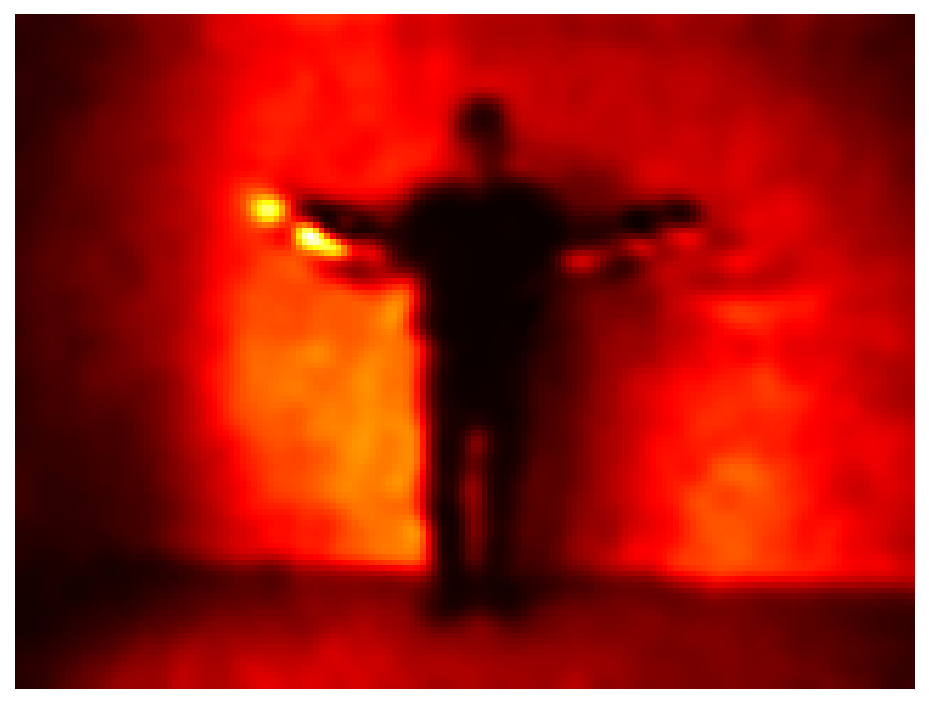
\includegraphics[width=\textwidth]{handclapping_gabor_s2_t1.5_thr0.1_frame42_H.png}
        \caption{frame 42}
    \end{subfigure}
    \caption{Gabor - handclapping: χάρτης ενέργειας $H$ (κλίμακα \textit{hot}).}
    \label{fig:gabor_H_handclapping}
\end{figure}

Παρατηρούμε ότι και οι δύο ανιχνευτές καταφέρνουν να εντοπίσουν σημεία
ενδιαφέροντος στις περιοχές κίνησης (χέρια, πόδια). Ωστόσο, υπάρχουν
σημαντικές διαφορές τόσο στον τύπο των σημείων που εντοπίζουν όσο και
στην πυκνότητά τους.

Ο Harris3D εντοπίζει σημεία σε περιοχές που παρουσιάζουν \emph{ταυτόχρονα}
χωρική δομή (γωνίες, άκρα) και χρονική μεταβολή.
Επικεντρώνεται κυρίως στα άκρα των άκρων και στα σύνορα σώματος–φόντου
όπου η τροχιά κίνησης προκαλεί αλλαγή εμφάνισης.
Τα σημεία που εντοπίζει τείνουν να είναι \emph{αραιά}: τόσο ο αριθμός των
frames με ανιχνεύσεις όσο και η πυκνότητα ανά frame είναι χαμηλότερα σε σχέση
με τον Gabor. Αυτό οφείλεται στο γεγονός ότι ο Harris3D απαιτεί και τα δύο
κριτήρια (χωρικό \emph{και} χρονικό) να ικανοποιούνται ταυτόχρονα.

Ο Gabor αντιδρά κυρίως στη χρονική μεταβολή, εντοπίζοντας περιοχές με
ρυθμικά επαναλαμβανόμενη κίνηση (ο ρυθμός ορίζεται από $\omega = 4/\tau$).
Είναι αισθητά πιο ευαίσθητος στις ανιχνεύσεις: σπάνια χάνει σημεία
ενδιαφέροντος σε frame που εμφανίζεται κινούμενο αντικείμενο.
Για \textit{handclapping} τα σημεία κατανέμονται πιο ομοιόμορφα κατά μήκος
της περιοχής κίνησης των χεριών, αντιδρώντας στην περιοδικότητα της δράσης.
Για \textit{walking} και \textit{running} εντοπίζει κυρίως τα άκρα λόγω της
μεγαλύτερης χρονικής τους μεταβολής.

Και οι δύο ανιχνευτές εντοπίζουν ευκολότερα έντονες κινήσεις
(π.χ.\ κίνηση γονάτων και αστραγάλων στο \textit{running})
από ό,τι πιο αργές (π.χ.\ βάδισμα).
Ωστόσο, είναι ικανοί να ανιχνεύσουν και πολύ μικρές μετακινήσεις σε
ορισμένες περιπτώσεις, όπως η ελαφρά μετακίνηση των ποδιών σε σκηνές
με χαμηλή κινητικότητα.

\subsection{Χωρο-χρονικοί Ιστογραφικοί Περιγραφητές}

Έχοντας εντοπίσει τα χωρο-χρονικά σημεία ενδιαφέροντος $(x_0, y_0, t_0, \sigma)$
στην προηγούμενη ενότητα, το επόμενο βήμα είναι η \emph{εξαγωγή
χαρακτηριστικών}, δηλαδή η μετατροπή της τοπικής γειτονιάς κάθε σημείου σε ένα
διάνυσμα σταθερής διάστασης που περιγράφει τι συμβαίνει γύρω από το
σημείο. Για τον σκοπό αυτό χρησιμοποιούνται δύο τοπικοί
περιγραφητές που συμπληρώνουν ο ένας τη λειτουργία του άλλου, οι \textbf{HOG} (Histogram of Oriented Gradients) και
\textbf{HOF} (Histogram of Optical Flow), ακολουθώντας τους
Laptev et al.~\cite{laptev2008} που τους εισήγαγαν ως επέκταση του κλασικού
SIFT.
Η δύναμη της σύζευξης βρίσκεται στο γεγονός ότι ο
HOG αποτυπώνει τη στιγμιαία \emph{εμφάνιση} (στάση σώματος, περίγραμμα
μελών), ενώ ο HOF την \emph{κίνηση} (κατεύθυνση και ένταση μετατοπίσεων).

Ο \textbf{HOG} (Histogram of Oriented Gradients), όπως είδαμε και στο
προηγούμενο εργαστήριο, κωδικοποιεί τη χωρική δομή (ακμές, περιγράμματα,
υφές) μέσω του gradient της έντασης: για κάθε pixel υπολογίζει τις
μερικές παραγώγους $G_x, G_y$, εξάγει γωνία και μέτρο, και φτιάχνει
ιστόγραμμα των γωνιών σταθμισμένο με το μέτρο. Αποτυπώνει έτσι τη
\emph{στιγμιαία γεωμετρία} του σώματος (στάση κορμού, θέση χεριών και
ποδιών, σιλουέτα), που συχνά αρκεί από μόνη της για να ξεχωρίσει
δράσεις όπως \textit{handclapping} με ανυψωμένα χέρια έναντι
\textit{walking} με χέρια στα πλάγια.

Ο \textbf{HOF} (Histogram of Optical Flow) κωδικοποιεί αντί για γεωμετρία
την \emph{κίνηση} γύρω από το σημείο. Για κάθε ζεύγος διαδοχικών frames
υπολογίζεται πεδίο οπτικής ροής $(f_x, f_y)$ που εκτιμά πόσο και προς
ποια κατεύθυνση μετακινήθηκε κάθε pixel, και στη συνέχεια κατασκευάζεται
ιστόγραμμα των κατευθύνσεων σταθμισμένο με το μέτρο της ροής (ώστε
ασθενείς, θορυβώδεις μετατοπίσεις να μη κυριαρχούν). Το ιστόγραμμα αυτό
απομονώνει την κίνηση από την εμφάνιση και είναι ιδιαίτερα διακριτικό
για περιοδικές δράσεις όπως \textit{walking} ή \textit{running}, όπου
διαφορετικές φάσεις του κύκλου παράγουν χαρακτηριστικές κατανομές ροής.

Σημειώνουμε ότι στο paper των Laptev et al.\ ο τοπικός όγκος έχει
διαστάσεις $\Delta x, \Delta y = 2k\sigma$, $\Delta t = 2k\tau$ με $k{=}9$,
και υποδιαιρείται σε πλέγμα $(n_x, n_y, n_t) = (3, 3, 2)$ cuboids. Στη
δική μας υλοποίηση αποκλίνουμε συνειδητά από αυτές τις τιμές: ο όγκος
γίνεται \emph{χωρικός} ($n_t{=}1$) με πλέγμα $3\times3$ και πλευρά
$4\sigma$ (δηλαδή $k{=}2$), ώστε ο περιγραφητής να παραμένει συμπαγής
$144$-d (αντί να κλιμακωθεί σε $432$-d από τα $2\!\times\!3\!\times\!3$
cuboids του paper) και να κρατήσουμε χαμηλό το υπολογιστικό κόστος σε
ολόκληρο το pipeline — οι δοκιμές μας έδειξαν ότι η μείωση του patch
δεν βλάπτει σημαντικά την τελική ακρίβεια.

\subsubsection{Υπολογισμός Gradient και Οπτικής Ροής}

Όσον αφορά τον υπολογισμό των περιγραφητών \textbf{HOG} για κάθε frame $t$ υπολογίζονται οι οριζόντιες και κατακόρυφες συνιστώσες της
βαθμίδας έντασης μέσω κεντρικών διαφορών:
\begin{equation}
    G_x = I \ast [-1,\;0,\;1], \qquad G_y = I \ast [-1,\;0,\;1]^\top
\end{equation}
Η χρήση κεντρικών διαφορών (αντί Sobel) είναι συμβατή με τον τρόπο που
υπολογίστηκαν οι παράγωγοι στους ανιχνευτές, εξασφαλίζοντας συνέπεια κλίμακας.

Από την άλλη όσον αφορά τον υπολογισμό των περιγραφητών \textbf{HOF}, για κάθε ζεύγος διαδοχικών frames $(t, t{+}1)$ υπολογίζεται πεδίο οπτικής ροής
$(f_x, f_y)$ μέσω του αλγορίθμου \textbf{TV-L1}. Το TV-L1 παράγει πυκνή ροή
με ισχυρή αντοχή σε θόρυβο και στα άλματα έντασης χάρη στον όρο ολικής
μεταβολής. Χρησιμοποιήθηκε η υλοποίηση του OpenCV μέσω της \texttt{cv2.optflow.DualTVL1OpticalFlow\_create(nscales=1)} που υπολογίζει τη ροή σε μία μόνο κλίμακα, αποφεύγοντας την πυραμίδα που θα αύξανε σημαντικά τον υπολογιστικό φόρτο.

\subsubsection{Εξαγωγή HOG/HOF Περιγραφητών}

Αφού έχουν προϋπολογιστεί τα πεδία $G_x$, $G_y$ και η οπτική ροή
$(f_x, f_y)$ για όλα τα frames του βίντεο, η εξαγωγή των περιγραφητών
γίνεται \emph{ανά σημείο ενδιαφέροντος}. Για κάθε σημείο
$(x_0, y_0, t_0, \sigma)$ που επιστράφηκε από τον ανιχνευτή, ορίζεται ένα
τετράγωνο χωρικό παράθυρο (\emph{patch}) πλευράς $4\sigma$ pixels γύρω από
τη θέση του, δηλαδή
$[y_0 - 2\sigma,\, y_0 + 2\sigma] \times [x_0 - 2\sigma,\, x_0 + 2\sigma]$,
πάνω στο frame $t_0$. Η σύνδεση του μεγέθους του patch με την κλίμακα
$\sigma$ του ανιχνευτή εξασφαλίζει ότι ο περιγραφητής αποτυπώνει την
τοπική δομή στην \emph{ίδια κλίμακα} στην οποία εντοπίστηκε το σημείο.
Το patch αποκόπτεται στα όρια της εικόνας για να αποφευχθεί έξοδος εκτός
ορίων, και εκφυλισμένα patches (διαστάσεων μικρότερων των $2$ pixels) που
μπορεί να προκύψουν για σημεία πολύ κοντά στο περιθώριο παραλείπονται από την υλοποίηση μας.

Πάνω σε κάθε τέτοιο patch εφαρμόζεται η έτοιμη συνάρτηση
\texttt{orientation\_histogram} του δοσμένου υλικού, η οποία είναι
γενική και δέχεται οποιοδήποτε διανυσματικό πεδίο $(u, v)$ πάνω στο
patch· ανάλογα με το τι της τροφοδοτούμε, παράγεται είτε HOG είτε HOF.
Εσωτερικά, η συνάρτηση υποδιαιρεί το patch σε πλέγμα $3\times 3$ κελιών
και σε κάθε κελί φτιάχνει ιστόγραμμα $8$ bins με βάση τη γωνία του
$(u, v)$ κάθε pixel, σταθμισμένο με το μέτρο του $\sqrt{u^2+v^2}$
— έτσι ώστε ισχυρά διανύσματα (έντονες ακμές ή γρήγορη κίνηση) να
μετρούν περισσότερο από θορυβώδη. Τα εννέα $8$-d ιστογράμματα
συνενώνονται σε ένα $3\!\times\!3\!\times\!8 = 72$-διάστατο υπο-διάνυσμα.

Η υλοποίηση μας καλεί τη συνάρτηση δύο φορές ανά σημείο, πάνω στο ίδιο
patch. Για τον \textbf{HOG} τροφοδοτούνται οι χωρικές βαθμίδες
$(G_x, G_y)$ του frame $t_0$, οπότε το ιστόγραμμα αποτυπώνει τις
κατευθύνσεις των τοπικών ακμών, δηλαδή τη γεωμετρική δομή (περιγράμματα
μελών, στάση σώματος). Για τον \textbf{HOF} τροφοδοτούνται οι
συνιστώσες της οπτικής ροής $(f_x, f_y)$ μεταξύ των frames $t_0$ και
$t_0{+}1$, οπότε τώρα το ιστόγραμμα αποτυπώνει τις κατευθύνσεις και τις
εντάσεις της τοπικής κίνησης. Αν το σημείο ενδιαφέροντος εντοπιστεί
στο τελευταίο frame όπου δεν υπάρχει εμπρόσθια ροή, χρησιμοποιείται
μηδενικό πεδίο.

Τα δύο $72$-d υπο-διανύσματα συνενώνονται σε έναν ενιαίο περιγραφητή
$144$ διαστάσεων $[\text{HOG}\,\|\,\text{HOF}]$, με τις πρώτες $72$
θέσεις να αντιστοιχούν στην εμφάνιση και τις υπόλοιπες $72$ στην
κίνηση. Η διάταξη αυτή επιλέχθηκε συνειδητά ώστε στην Εν.~2.3 να
μπορούμε να αξιολογήσουμε ξεχωριστά κάθε υπο-περιγραφητή κρατώντας
απλώς τις πρώτες ή τις τελευταίες $72$ στήλες του πίνακα περιγραφητών.

\subsection{Κατασκευή Bag of Visual Words και Ταξινόμηση με SVM}

Έχοντας πλέον για κάθε βίντεο ένα σύνολο $144$-διάστατων περιγραφητών,
το επόμενο βήμα είναι η ταξινόμησή του σε μία από τις τρεις δράσεις. Το
πλήθος των περιγραφητών διαφέρει από βίντεο σε βίντεο, οπότε πρέπει
πρώτα να μετατραπούν σε αναπαράσταση σταθερής διάστασης.

Για τον σκοπό αυτό χρησιμοποιούμε την προσέγγιση \textbf{Bag of Visual
Words (BoVW)}. Με K-means πάνω στους περιγραφητές εκπαίδευσης χτίζουμε
ένα λεξιλόγιο $K$ \emph{visual words} (κεντροειδών), και στη συνέχεια
κάθε βίντεο κωδικοποιείται σε ένα κανονικοποιημένο ιστόγραμμα που μετράει
πόσες φορές εμφανίζεται η κάθε οπτική λέξη στους περιγραφητές του.

Με αυτό το ιστόγραμμα ως είσοδο, εκπαιδεύουμε έναν $\chi^2$-SVM
ταξινομητή μέσω της έτοιμης συνάρτησης \texttt{svm\_train\_test} του
\texttt{cv26\_lab2\_utils.py}.

\subsubsection{Διαχωρισμός Συνόλου Δεδομένων}

Ο διαχωρισμός των βίντεο σε σύνολα εκπαίδευσης και ελέγχου ορίζεται από
το αρχείο \texttt{traininng\_videos.txt} που συνοδεύει το dataset.
Διαβάζουμε τα ονόματα που περιέχει, συλλέγουμε όλα τα \texttt{.avi} από
τους φακέλους των τριών δράσεων (\textit{walking}, \textit{running},
\textit{handclapping}), και χωρίζουμε σε $36$ βίντεο εκπαίδευσης και $12$
βίντεο ελέγχου ανάλογα με το αν το όνομα κάθε αρχείου περιλαμβάνεται ή
όχι στη λίστα. Από κάθε βίντεο φορτώνουμε τα πρώτα $100$ καρέ σε
αποχρώσεις του γκρι, μέσω της συνάρτησης \texttt{read\_video}.

\subsubsection{Κατασκευή Λεξιλογίου visual words}

Για την κωδικοποίηση κάθε βίντεο σε ένα ιστόγραμμα visual words
χρησιμοποιούμε τη συνάρτηση \texttt{bag\_of\_words} του
\texttt{cv26\_lab2\_utils.py}. Η κλήση γίνεται ως
\texttt{bow\_tr, bow\_ts = bag\_of\_words(tr, ts, num\_centers=K)}, όπου
\texttt{tr} και \texttt{ts} είναι λίστες μήκους ίσου με τον αριθμό των
train και test βίντεο αντίστοιχα, και κάθε στοιχείο τους είναι ένας
δισδιάστατος πίνακας με έναν περιγραφητή ανά γραμμή. Η παράμετρος
\texttt{num\_centers} ορίζει το πλήθος $K$ των κεντροειδών του K-means,
δηλαδή το μέγεθος του λεξιλογίου. Εσωτερικά η συνάρτηση τρέχει K-means
μόνο στους περιγραφητές εκπαίδευσης (χρησιμοποιώντας τυχαίο δείγμα $50\%$
για ταχύτητα) και μετά κβαντίζει κάθε περιγραφητή κάθε βίντεο στο
πλησιέστερο κεντροειδές, επιστρέφοντας $\ell_2$-κανονικοποιημένα
ιστογράμματα συχνοτήτων.

Στη δική μας υλοποίηση καλούμε την \texttt{bag\_of\_words} μέσα σε έναν
βρόχο που διατρέχει διαφορετικούς συνδυασμούς ανιχνευτή (Harris, Gabor,
ή το union των δύο), τύπου περιγραφητή (HOG, HOF, ή HOG/HOF) και
μεγέθους λεξιλογίου. Για τα πειράματα που χρησιμοποιούν μόνο έναν
υπο-περιγραφητή, αρκεί να κρατήσουμε τις πρώτες ή τις τελευταίες $72$
στήλες κάθε πίνακα περιγραφητών (\texttt{d[:, :72]} για HOG,
\texttt{d[:, 72:]} για HOF) πριν την κλήση, αξιοποιώντας τη διάταξη
$[\text{HOG}\,\|\,\text{HOF}]$ που επιβάλαμε στο 2.2.2. Ως μέγεθος
λεξιλογίου δοκιμάζουμε στα τελικά μας πειράματα $K \in \{50, 100, 200\}$, ώστε να αξιολογήσουμε
την επίδραση της χωρητικότητας του λεξιλογίου στην τελική ακρίβεια.

\subsubsection{Ταξινόμηση με SVM}

Αφού έχουμε για κάθε βίντεο ένα $K$-διάστατο ιστόγραμμα BoVW, το
ταξινομούμε σε μία από τις τρεις δράσεις μέσω της έτοιμης συνάρτησης
\texttt{svm\_train\_test(bow\_tr, train\_labels, bow\_ts, test\_labels)}
του \texttt{cv26\_lab2\_utils.py}. Η συνάρτηση επιστρέφει την ακρίβεια
στο test set και τις προβλέψεις ανά βίντεο.

Εσωτερικά η \texttt{svm\_train\_test} χρησιμοποιεί έναν SVM με πυρήνα
$\chi^2$, ο οποίος είναι καταλληλότερος για ιστογράμματα από τον απλό
γραμμικό ή τον RBF. Ο πυρήνας έχει τη μορφή
\begin{equation}
    K_{\chi^2}(\mathbf{x}, \mathbf{y}) =
    \exp\!\left(-\gamma \sum_i \frac{(x_i - y_i)^2}{x_i + y_i}\right),
\end{equation}
όπου ο παρονομαστής $x_i + y_i$ δίνει μεγαλύτερη βαρύτητα σε bins με
μικρές τιμές, αποτρέποντας τις λίγες κυρίαρχες οπτικές λέξεις να
επιβληθούν στη μέτρηση ομοιότητας — κάτι που θα συνέβαινε με την απλή
ευκλείδεια απόσταση. Πρακτικά ο πίνακας του πυρήνα υπολογίζεται εκ των
προτέρων (\texttt{precomputed}) και κανονικοποιείται διαιρούμενος με τη
μέση τιμή του, ώστε η κλίμακα των αποστάσεων να μην εξαρτάται από το
μέγεθος του λεξιλογίου.

Επειδή οι δράσεις είναι τρεις και το SVM είναι εκ φύσεως δυαδικός
ταξινομητής, η \texttt{svm\_train\_test} εκπαιδεύει εσωτερικά τρία
ανεξάρτητα SVMs με στρατηγική \emph{One-vs-Rest}: το καθένα μαθαίνει να
διακρίνει μία κλάση από τις υπόλοιπες δύο. Για κάθε test βίντεο
επιλέγεται η κλάση με τη μεγαλύτερη πιθανότητα (μέσω Platt scaling), και
η τελική ακρίβεια υπολογίζεται ως το ποσοστό σωστών προβλέψεων στα $12$
test βίντεο.

\subsubsection{Πειραματισμοί και Σχολιασμός}

Τρέξαμε συνολικά $27$ πειράματα ώστε να δούμε πώς επηρεάζουν την τελική
ακρίβεια οι επιλογές ανιχνευτή (Harris3D, Gabor ή η ένωσή τους), τύπου
περιγραφητή (HOG, HOF ή HOG+HOF) και οι υπερπαράμετροι $\sigma$, $\tau$,
$\theta$, $N$ και $K$. Στα πειράματα με την ένωση ανιχνευτών συνενώνουμε
απλά τους περιγραφητές Harris και Gabor κάθε βίντεο πριν το BoVW. Για
τις παραλλαγές HOG / HOF αξιοποιούμε τη διάταξη $[\text{HOG}\|\text{HOF}]$
του $144$-d διανύσματος και κρατάμε τις πρώτες ή τις τελευταίες $72$
στήλες, χωρίς να ξαναϋπολογίζουμε περιγραφητές. Τα αποτελέσματα όλων των
πειραμάτων συνοψίζονται στον Πίνακα~\ref{tab:results}.

\begin{table}[H]
\centering
\caption{Αποτελέσματα πειραμάτων. Ακρίβεια ταξινόμησης στο σύνολο ελέγχου
(12 βίντεο). Βέλτιστες τιμές επισημαίνονται με \textbf{έντονη γραφή}.}
\label{tab:results}
\setlength{\tabcolsep}{5pt}
\begin{tabular}{llcccccc}
\toprule
\textbf{Ανιχνευτής} & \textbf{Περιγρ.} & $\boldsymbol{\sigma}$ & $\boldsymbol{\tau}$ & $\boldsymbol{\theta}$ & $\boldsymbol{N}$ & $\boldsymbol{K}$ & \textbf{Ακρίβεια} \\
\midrule
\multicolumn{8}{l}{\textit{Βασικά πειράματα (detector \& descriptor type)}} \\
harris       & HOG+HOF & 1 & 0.7 & 0.1  & 500  & 50  & 50.00\% \\
harris       & HOG     & 1 & 0.7 & 0.1  & 500  & 50  & 58.33\% \\
harris       & HOG+HOF & 2 & 1.5 & 0.1  & 500  & 50  & 75.00\% \\
gabor        & HOG+HOF & 2 & 1.5 & 0.1  & 500  & 50  & 75.00\% \\
gabor        & HOG     & 2 & 1.5 & 0.1  & 500  & 50  & 75.00\% \\
gabor        & HOF     & 2 & 1.5 & 0.1  & 500  & 50  & 75.00\% \\
harris       & HOG     & 2 & 1.5 & 0.1  & 500  & 50  & 75.00\% \\
harris       & HOF     & 2 & 1.5 & 0.1  & 500  & 50  & 83.33\% \\
harris+gabor & HOG+HOF & 2 & 1.5 & 0.1  & 500  & 50  & 83.33\% \\
\midrule
\multicolumn{8}{l}{\textit{Μέγεθος λεξιλογίου $K$ (gabor baseline)}} \\
gabor        & HOG+HOF & 2 & 1.5 & 0.1  & 500  & 100 & \textbf{91.67\%} \\
gabor        & HOG+HOF & 2 & 1.5 & 0.1  & 500  & 200 & 75.00\% \\
\midrule
\multicolumn{8}{l}{\textit{Χωρική κλίμακα $\sigma$}} \\
gabor        & HOG+HOF & 3 & 1.5 & 0.1  & 500  & 50  & 66.67\% \\
gabor        & HOG+HOF & 4 & 1.5 & 0.1  & 500  & 50  & 66.67\% \\
harris       & HOG+HOF & 4 & 1.5 & 0.1  & 500  & 50  & 41.67\% \\
\midrule
\multicolumn{8}{l}{\textit{Χρονική κλίμακα $\tau$}} \\
harris       & HOG+HOF & 2 & 1.0 & 0.1  & 500  & 50  & 33.33\% \\
gabor        & HOG+HOF & 2 & 1.0 & 0.1  & 500  & 50  & 41.67\% \\
gabor        & HOG+HOF & 2 & 2.0 & 0.1  & 500  & 50  & 33.33\% \\
\midrule
\multicolumn{8}{l}{\textit{Κατώφλι $\theta$}} \\
gabor        & HOG+HOF & 2 & 1.5 & 0.05 & 500  & 50  & 83.33\% \\
gabor        & HOG+HOF & 2 & 1.5 & 0.2  & 500  & 50  & 75.00\% \\
gabor        & HOG+HOF & 2 & 1.5 & 0.3  & 500  & 50  & 66.67\% \\
harris       & HOG+HOF & 2 & 1.5 & 0.05 & 500  & 50  & 83.33\% \\
\midrule
\multicolumn{8}{l}{\textit{Πλήθος σημείων $N$ και εναλλαγή $Κ$ (gabor)}} \\
gabor        & HOG+HOF & 2 & 1.5 & 0.1  & 200  & 50  & 66.67\% \\
gabor        & HOG+HOF & 2 & 1.5 & 0.1  & 1000 & 50  & \textbf{91.67\%} \\
gabor        & HOG     & 2 & 1.5 & 0.1  & 1000 & 50  & 83.33\% \\
gabor        & HOG+HOF & 2 & 1.5 & 0.1  & 1000 & 100 & 83.33\% \\
gabor        & HOG+HOF & 2 & 1.5 & 0.1  & 1000 & 200 & 66.67\% \\
gabor        & HOG+HOF & 2 & 1.5 & 0.1  & 2000 & 50  & 75.00\% \\
\bottomrule
\end{tabular}
\end{table}

Στο baseline ($\sigma{=}2$, $\tau{=}1.5$, $\theta{=}0.1$, $N{=}500$,
$K{=}50$) οι δύο ανιχνευτές πετυχαίνουν την ίδια ακρίβεια $75\%$, ενώ
η ένωσή τους (\texttt{harris+gabor}) ανεβαίνει στο $83.33\%$. Το
πλεονέκτημα του Gabor εμφανίζεται μόνο όταν ρυθμίσουμε το λεξιλόγιο ή
την πυκνότητα σημείων: με $K{=}100$ (ή εναλλακτικά με $N{=}1000$
διατηρώντας $K{=}50$) φτάνει στο $91.67\%$, τη μέγιστη ακρίβεια όλων των
πειραμάτων μας. Ενδιαφέρον εύρημα είναι ότι για τον Harris ο
περιγραφητής HOF μόνος του ($83.33\%$) υπερτερεί του συνδυασμένου
HOG+HOF ($75\%$), πιθανώς επειδή η χρονική πληροφορία βοηθάει τον
Harris να αντισταθμίσει τη χωρική του ευαισθησία.

Όσον αφορά τους υπο-περιγραφητές για τον Gabor, και οι τρεις
παραλλαγές (HOG, HOF, HOG+HOF) δίνουν στο baseline $75\%$· διαφορά
υπέρ του HOG+HOF εμφανίζεται όταν αυξάνουμε την πυκνότητα σημείων:
για $N{=}1000, K{=}50$ ο συνδυασμένος HOG+HOF φτάνει $91.67\%$ ενώ ο
HOG μόνο $83.33\%$. Αυτό υποδεικνύει ότι εμφάνιση και κίνηση είναι
\emph{συμπληρωματικές} ειδικά για τον Gabor detector, όταν υπάρχουν
αρκετά σημεία ώστε τα μοτίβα στάσης και κίνησης να κωδικοποιηθούν
ξεχωριστά.

Όσον αφορά το μέγεθος του λεξιλογίου $K$: για $N{=}500$, το $K{=}50$ δίνει $75\%$, το $K{=}100$ πηδά στο
$91.67\%$, και το $K{=}200$ επιστρέφει στο $75\%$. Το $K{=}50$ φαίνεται
να συγχωνεύει διαφορετικά κινητικά μοτίβα στα ίδια bins, ενώ το
$K{=}200$ υπερ-εξειδικεύεται και παράγει πολύ αραιά ιστογράμματα. Όταν
αυξάνεται το $N$ στα $1000$ η συμπεριφορά αντιστρέφεται: τώρα το
$K{=}50$ είναι το βέλτιστο ($91.67\%$) και η αύξηση του $K$ οδηγεί σε
πτώση ($83.33\%$ για $K{=}100$, $66.67\%$ για $K{=}200$) — με
περισσότερα σημεία ανά βίντεο, ένα μικρό λεξιλόγιο είναι ήδη στατιστικά
επαρκές.

Η χρονική κλίμακα $\tau$ είναι η πιο ευαίσθητη παράμετρος. Το
$\tau{=}1.0$ ρίχνει την ακρίβεια στο $41.67\%$ και το $\tau{=}2.0$ στο
$33.33\%$, πολύ κάτω από το $75\%$ του $\tau{=}1.5$. Στενό χρονικό
παράθυρο δεν προλαβαίνει να «δει» την περιοδικότητα των δράσεων, ενώ
πολύ φαρδύ παίρνει μέσο όρο πολλών φάσεων και χάνει τη χρονική δομή. Η
$\tau{=}1.5$ επιβεβαιώνεται πειραματικά ως η σωστή χρονική κλίμακα για
τις δράσεις του KTH.

Η χωρική κλίμακα $\sigma$ είναι πιο ήπια αλλά παρόμοια στη συμπεριφορά:
η τιμή $\sigma{=}2$ είναι βέλτιστη, ενώ για $\sigma{=}3$ και $\sigma{=}4$
ο Gabor πέφτει στο $66.67\%$. Ο Harris είναι ακόμα πιο ευαίσθητος στο
$\sigma$: στο $\sigma{=}4$ καταρρέει στο $41.67\%$, υποδεικνύοντας ότι
το υπερβολικό smoothing καταστρέφει τις χωρο-χρονικές γωνιακότητες που
αναζητά.

Το κατώφλι $\theta$ παρουσιάζει μονότονη συμπεριφορά: μικρότερο
κατώφλι σημαίνει περισσότερα (και πιο φτωχά) σημεία, μεγαλύτερο σημαίνει
λιγότερα και πιο ισχυρά. Το $\theta{=}0.05$ δίνει $83.33\%$ τόσο για τον
Gabor όσο και για τον Harris — για τον Harris μάλιστα αυτή είναι η
καλύτερη ρύθμιση όταν χρησιμοποιείται HOG+HOF. Αυξάνοντας το $\theta$ η
ακρίβεια πέφτει ομαλά ($75\%$ στο $0.2$, $66.67\%$ στο $0.3$).

Το πλήθος σημείων $N$ ακολουθεί επίσης καμπύλη με κορυφή: $N{=}200$
δίνει $66.67\%$, $N{=}500$ δίνει $75\%$, $N{=}1000$ πετυχαίνει $91.67\%$,
ενώ $N{=}2000$ επιστρέφει στο $75\%$. Το $N{=}1000$ αντιπροσωπεύει το
σημείο όπου τα σημεία είναι αρκετά για να καλύψουν πλούσια τις δράσεις
αλλά όχι τόσα ώστε να αρχίσουν να επιλέγονται από αδιάφορες περιοχές
του φόντου.

Δοκιμάσαμε τέλος τον Harris με τις παραμέτρους αναφοράς των Laptev et
al.\ ($\sigma{=}1$, $\tau{=}0.7$): η ακρίβεια πέφτει στο $50\%$ (HOG+HOF)
και στο $58.33\%$ (HOG), πολύ χαμηλότερα από τη δική μας ρύθμιση
$\sigma{=}2, \tau{=}1.5$. Αυτό δείχνει ότι οι τιμές του paper δεν
μεταφέρονται αυτόματα στο δικό μας υποσύνολο με μόνο τους πρώτους $100$
frames, και επιβεβαιώνει την ανάγκη βαθμονόμησης ανά dataset.

Ο καλύτερος συνδυασμός του πειράματός μας είναι ο Gabor ανιχνευτής με
HOG+HOF περιγραφητές, $\sigma{=}2$, $\tau{=}1.5$, $\theta{=}0.1$, και
είτε $N{=}500$ με $K{=}100$, είτε $N{=}1000$ με $K{=}50$. Η ακρίβεια
$91.67\%$ είναι πρακτικά ίδια με το $91.8\%$ που αναφέρουν οι Laptev et
al.\ στο πλήρες KTH με BoF$+\chi^2$-SVM, αν και εμείς την πετυχαίνουμε
με μονο-κλιμακωτή ανίχνευση και μικρό λεξιλόγιο — δικαιολογημένο από το
ότι το δικό μας υποσύνολο έχει $3$ κλάσεις αντί $6$ και ισοζυγισμένα
splits.

% ─────────────────────────────────────────────────────────────────────────────
\section{Ταξινόμηση Βίντεο με Χρήση Προεκπαιδευμένων Βαθιών Νευρωνικών Δικτύων}

\subsection{2D Χαρακτηριστικά με MobileNet}

\subsubsection{Φόρτωση Βίντεο UCF11}

% TODO

\subsubsection{Εξαγωγή Χαρακτηριστικών με MobileNet\_v3\_small}

% TODO

\subsubsection{Ταξινόμηση με SVM}

% TODO

\subsection{3D Χαρακτηριστικά με x3d\_xs}

\subsubsection{Φόρτωση Μοντέλου x3d\_xs}

% TODO

\subsubsection{Εξαγωγή Χαρακτηριστικών και Προετοιμασία Δεδομένων}

% TODO

\subsubsection{Ταξινόμηση και Confusion Matrix}

% TODO

\subsubsection{Σύγκριση 2D και 3D Προσεγγίσεων}

% TODO

% ─────────────────────────────────────────────────────────────────────────────
\begin{thebibliography}{9}

\bibitem{laptev2008}
I.~Laptev, M.~Marszalek, C.~Schmid, and B.~Rozenfeld,
``Learning realistic human actions from movies,''
in \textit{Proc. IEEE CVPR}, pp.~1-8, 2008.

\bibitem{laptev2003}
I.~Laptev and T.~Lindeberg,
``Space-time interest points,''
in \textit{Proc. IEEE ICCV}, vol.~1, pp.~432-439, 2003.

\end{thebibliography}

\end{document}
